\documentclass[fleqn,twocolumn]{mynote}

\begin{document}
\title{卒業研究ノート}
\author{中村 龍造}
\date{}
\maketitle

\section*{2024-07-20}
研究生活が始まって半年ながら,研究ノートをとってみようと思う.といっても,研究にまつわる日記のような感じで使おうと思っている.なのでその日の研究に関することを中心に,いろいろメモしていこうと思う.

今日は卒論の修正リストを作った.はじめはめちゃくちゃ赤入れられてショックだったが,数えてみるとそんなに多くもないので,なんだか行けそうな気がする.13個くらい.はじめてちゃんと書いたにしては少ないんじゃないか.バグの数だと思えば.

卒論修正リストを参考に,土日は卒論を直して,できれば日曜の午後くらいには佐藤先生にまた提出したいと思っている.懸念点としては,参考文献のいりそうな修正項目がいくつかあるということ.たぶん今回の修正項目,大まかに分けると,1. 参考文献を盛る,2. 内容を面白くする,の2つに分かれる.1は1章2章で,2は3章の構想で必要になる.参考文献をじっくり読み漁る時間も無いので,そのへんは美味いことバランスを取ったほうがいいかもと思ったが,どっちも半分くらいやったらいいんじゃないかと思う.

いまから久しぶり(6日ぶり)によわtoioシステムのほうをいじくる.改めて振り返ったら,プロトタイピングをしていないのがおれだけだったのでなんだか嫌な気分.「大学は失敗をたくさんするための場」とよく言われるが,その点ではおれが一番学びを活かせていないのかもしれない.だって失敗すると「あいつはしょぼいやつなんだな」って思われそうで嫌なんだもん.失敗すればするほど嫌なことしか積み重ならない.今回がはじめての「良い失敗」を積み重ねる機会になるか.

さて,ではよわtoio(仮称)を実装していく.とはいえ設計だけは以前のおれがそれなりにやってくれている.いまのおれがするのはそれを形にすること.目標は\textbf{「何らかの環境データを取得したtoioに何らかの反応を取らせること」}.

今回やることは次の4個
\begin{enumerate}
  \item toioとUnityの接続の確認
  \item M5とUnityの接続の確認
  \item Unityでもらってきたデータをまとめるまでの流れをつくる
  \item まとめたデータを評価クラスで「評価」してみる
\end{enumerate}

\subsection*{toioとUnityの接続の確認}
接続方法は知る限り2通り.1つはBLE(Bluetooth Low Energy)接続をする方法,もう1つはSampleConnectTypeコンポーネントを追加し,ConnectTypeをRealに変更する方法.どちらも試してみたけど,接続までの速度も変わらないようなので,実装が楽な2つめの方法で行こうと思う.

この方法を使うと,Unity上のtoioにさせた動きを現実空間上のtoioにも反映させてくれる.なので仮想空間のtoioを相手にシステムを組んでさえいれば,自然と現実空間システムも組めているという寸法.便利.

今始めて知ったんだが,\LaTeX はアンダーバーを処理できないらしい.特殊文字なんだね.半角のカッコはおそらく英語圏でも使われるから普通に使えたのが罠だった.

\subsection*{M5とUnityの接続の確認}
toioの接続が無事完了して,今後の接続方式も固まったので,次にM5の確認.前にボードの違いでエラーが生じたが,正しいのを選べば今回も無事に通過.USB経由でデータが送られていることも確認できた.

キーボードガタガタ打つのも楽しいが,大量に入力する場合は面倒なのでPCでも音声入力ができないか調べてみた.どうやらいけるらしい.\\
\url{https://x.gd/3VbTT}

さて,音声入力をやっている.意外と精度が良いのかもしれこれでキーボードの代わりに音声入力ができるようになれば万々歳.

以前やっていた時にも感じていたが,M5とBluetoothの接続は手作業でやらなければいけないのが非常に面倒.が,確認してみたらBluetooth設定のCOMポートから名前まで見ることができるようなので楽できそう.

\begin{figure}[h]
  \label{bluetooth_com_port}
  \centering
  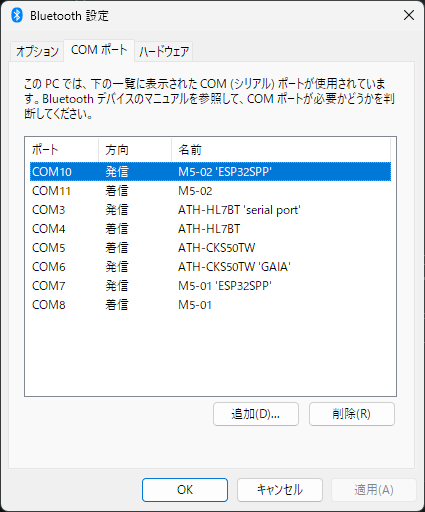
\includegraphics[keepaspectratio, width=0.7\columnwidth]{resources/bluetooth-connect.png}
  \caption[short]{Bluetooth設定の画面.COMポートタブではBluetooth接続されているデバイスのポート,方向,名前を見ることができ,手作業での接続が楽になりそう.}
\end{figure}

ここからさらにCOMポート設定をさらってデバイス名と同じ名前のCOMポートを自動で接続するようにすれば,更に楽になるかもしれない.\\
\url{https://qiita.com/ta-oot/items/2d74409cca729629595e}

Bluetoothでの入力が確認できたら,Unity側での設定は慣れたもの.COMポートも以前より安全に確認できるようになったので,設定も簡単.念のためUSBのポートも確認をしておけば安全.

そういえば忘れていたけれど,いまのプログラムだとBluetooth通信に失敗するとEditorがクラッシュするんだよね.困ったなあ.

あーきたきた.ようやく来た.

\begin{figure}[h]
  \label{m5-getting-sensor}
  \centering
  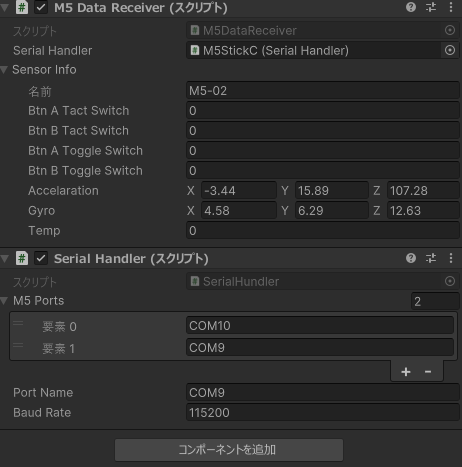
\includegraphics[keepaspectratio, width=0.7\columnwidth]{resources/m5stickc_getting_sensor.png}
  \caption[short]{UnityにM5StickCのデータが届いている様子.M5 Data Receiverはデータを受け取り,Serial HundlerはBluetoothシリアル通信の処理を担っている(らしい)}
\end{figure}

はじめCOM11,10,9を登録してたんだけど,検証したらCOM11はデータ送られてなかった.そのうえUnity側のボーレートも間違ってた.まあ直せる範囲のバグで良かったね.

よし,接続成功時はきちんとシーンも終わってくれる.一瞬「カクッ」っとなるのが恐怖を煽ってきていいよね.よくない.おめーなにクラッシュしてんだよ.絶対その不具合直すから.大方例外処理が不十分なんでしょうな.

\subsection*{本日のまとめ}
さて,なんだかんだ2時間ぐらい作業したので,今日の卒研は終了する.(みんなもっとやってるって?おれはおれの速度で進む.あとおれ脚質差しだから.巻き返すから,気合で.)

今回始めて\LaTeX で記録をつけてみたけれど,思ったより楽しい.なんだかリッチな見た目,リッチな書体で,まあ確かにメモを書くのには大仰というのも分かる.でもこの大仰さが,万年筆を使っているときのようなクセの強さと,それでしか得られない謎の快感があっていいな.癖になる.

今日はtoioおよびM5StickCの接続とデータの受け渡しを確認した.次回はtoioに付属しているセンサーの情報を取得する方法の調査と,取得データの集約まで進めたい.

\section*{2024.07.21}
卒論の修正を進めた.やっぱり思ったより時間がかかって,2時間でようやく3章がマシになったかならないかくらいの感じ.さらに赤が加わって,参考文献も必要になるのか.あと4日,間に合うかな……

ひとまず3章を直しきった次点で佐藤先生に共有した.もしかしたら「なんでこんな意味のないもの共有するんだろう?」とか思われてたら人間不信になって退学も辞さない.そういうこと考えるからおまえ「超危険メンヘラ」って言われるんだよ.

そういえばレビューコメントの扱い方,あれで良かったのかな?もしかしたら修正報告をして,向こうでResolveとかAcceptをするスタイルだったかもしれない.うーんわからん.まあなにか致命的にクソな使い方をしてる場合はきっと報告してくれるでしょう.よろ.

\section*{2024.07.23}
論文を添削に出したら全然できてないって怒られた上に「コメントちゃんと見えてる?」とかいう煽りを食らった.あらゆる憎しみを抑えて「ありがとうございます!」って返せたあのときのおれには今年最大級の称賛を送っていい.ああいう対応が今後も続くなら転ゼミも考慮する.佐藤クンは有能な人間が好きな感じがあるので,僕とは合わないとは思うけど.1年後にゼミレビューでボロクソにこき下ろすために耐えるか,苦しいのでお引越しするか.

恨みは尽きることがないので仕事の話をしよう.論文を直す.佐藤クンは実験風景を出せって言ってたけど,2日前で論文書き上がってないのに実験風景を作り出すってのは不可能.なので参考文献をあたって,論文としての品質を上げる

参考文献で知りたいこと

\begin{enumerate}
  \item ロボット高度化に対する姿勢たち \\ キーワードは
    \begin{enumerate}
      \item 関係論的なロボット(human-dependent robot)
      \item 社会的なロボット(social robot)
    \end{enumerate}
  \item 弱いロボット特有の活かすに値する特徴
  \item 弱いロボットの具体例
    \begin{enumerate}
      \item Muu
      \item ゴミ箱ロボット
      \item Talking Bone
      \item 岡田さん以外に弱いロボットやってる人の弱いロボット
      \item NICOBOもここで良さそう
    \end{enumerate}
  \item ロボットへの心理評価.印象,あるいは「はじめに」で述べたような「もっと高性能に」っていう要求が増えるのかどうか
  \item 「弱さ」の定量化手法
\end{enumerate}

\subsection*{ロボット高度化に対する姿勢たち}
\subsubsection*{STB: Human-Dependent Sociable Trash Box}
ゴミ箱ロボットの論文\cite{岡田美智男-2012-ゴミ箱ロ}.運良くACMに転がってた.social robotとhuman-dependent robotの定義の違いは掴んだ.

\begin{description}
  \item[social robot]\mbox{}\\
    ロボット自身の何らかの目標や動機を満たすために人々との社会的相互作用に参加するもの
  \item[human-dependent robot]\mbox{}\\
    人間の助けに依存して目標を達成する.KinzerのTweenbotが代表例.\\
    「あそこに行きたい」「これをして欲しい」という意図を示し,人間がそれを読み取ることでロボットの目標達成を助けてくれることが分かった.
\end{description}

したがって,social robotは目標達成に伴う行動を人と協働して行う.一方human-dependent robot は「こういう目標を達成したい」という意思表示のみを行い,それを見た人が自ずからロボットを助けてくれるようなロボットである\cite{Yamaji-2010-STBHumandependentSociableTrash}.こういう,周囲からの関与やアシストを引き出すことによる問題解決のやり方は赤子にも見られ,「関係論的な行為方略」と呼ばれる\cite{岡田美智男-2012-ゴミ箱ロ}.対立概念は「個体能力的な行為方略」と呼ばれ,個体として,自分ひとりで問題解決をするやり方をいう.

\section*{弱いロボット特有の強み}
これまでの流れ
\begin{description}
  \item[Social Robot]\mbox{}\\
    人とロボットどちらも目の前のタスクに関する目標を持っている\cite{Breazeal-2004-SocialInteractionsHRIRobot}.
  \item[Human-dependent Robot]\mbox{}\\
    ロボットだけが目標を持っている.何かしらの手段で目標を提示し,それを見た人間がロボットを助けてくれる.\\
    \Rightarrow 不特定多数の人間をタスク遂行のパートナーとすることができる\cite{--TweenbotsKacieKinzer}
  \item[弱いロボット]\mbox{}\\
    Human-dependent Robot の一種. \\
    Tweenbotとの違いは,目標の提示方法.Tweenbotは取り付けられた旗に書かれたテキストを読む.弱いロボットの1つであるゴミ箱ロボットは,動きと音声,タスクに関連した外観によって目標を読み取らせている.\\
\end{description}

\section{2024.07.24}

Notionに書いたプロットが大分イカしてたので転記する。

\subsection{はじめに}
\begin{itemize}
  \item Social Robot (Breazeal)\cite{Breazeal-2004-SocialInteractionsHRIRobot}: 「協働する人間とロボットは、それぞれタスクに関連した目標を持っている」
  \item Human-dependent Robot (Kinzer)\cite{--TweenbotsKacieKinzer}: 「ロボットのやりたいことを伝えられれば、そのへんの人間とも協働できるよね」
  \item 弱いロボット(関係論的なロボット)(岡田)\cite{岡田美智男-2012-ゴミ箱ロ}: 「やりたいことを効果的に伝えてサポートしてもらうために、赤ちゃんのテクニック(関係論的な行為方略)を使おう」
\end{itemize}
Human-dependent Robotから分かるのは、完全な自律性を持たなくとも、ロボットは現実世界の中で目標達成が可能であること
弱いロボットから分かるのは、Human-dependent Robotをデザインするときに、人間からのサポートを上手に引き出すテクニックがあること。(関係論的な行為方略)

\subsection{関連研究}
\begin{itemize}
  \item Sociable Trash Box\cite{Yamaji-2010-STBHumandependentSociableTrash}: 弱いロボットの好例
  \item INAMO\cite{岡田美智男-2012-ゴミ箱ロ}: 分散型エージェントは多数のロボットを同時に扱う必要がある。この研究は群ロボットに関係論的な行為方略を応用しようとしている。
\end{itemize}

課題: 既存の「弱いロボット」は、ハードウェア・ソフトウェアが強固に結びついてデザインされており、異なる目標に対する再利用性、異なる環境における適応力について課題がある。

コアとなるロボットはそのまま、要求に合わせてハードウェアを変えることで、ロボットが提供できる機能も変えているという例に、HERMITS\cite{Group-2020-HERMITS}がある。

自走用のモータを備えた小型ロボットエージェント(toio)に、「Shell」と呼ばれる交換可能なハードウェアを取り付けた研究。ハードウェアを変えることによって、掴む、持ち上げる、風を送る、などといった様々な機能をもたせることができている。

HERMITSでは、ハードウェアの交換によってロボットの役割を変えていた。本研究では、ロボットのセンシング及びアクションのプログラムの交換によって、異なる環境にも応用可能な弱いロボットを開発する。

\subsection{toioを操作できるようにする}
コントローラーの入力の扱われ方とか,サンプルコードとか
\url{https://hakonebox.hatenablog.com/entry/2018/04/15/125152}
\url{https://sorceryforce.net/ja/tips/unity-input-gamepad#toc7}

このアセットすごいよぉ!!
\url{https://assetstore.unity.com/packages/tools/input-management/controller-tester-43621}

TextMeshProで日本語を使う
\url{https://zenn.dev/kametani256/articles/63c083ab318136}
\url{https://gist.github.com/kgsi/ed2f1c5696a2211c1fd1e1e198c96ee4#file-japanese_full-txt}

ジョイスティックのシステムちょっと理解できた.

joystick button ~~ っていうのが押しボタン系.方向キー(Dpad)以外の押せるボタン一つ一つに番号が割り当てられてるので,ボタンごとの番号をチェックした後,ボタンの機能を割り当てればいい.

方向キーの扱いは,取りうる値が-1,0,1のジョイスティックっていう感じ.で,ジョイスティック側にもそういうのをいろいろ識別するために,「軸」が分けられてる.例えばLスティックは第1軸に割り当てられてる.方向キー左右は第7軸.なので例えば方向キーとアナログスティックで同じ動きをさせたいなら,7,8軸で値取るようにしたうえで,サブボタンにアナログスティックを割り当てる?

\section*{2024.07.25}
うおおおおおお先人ありがとーーーー!!!!!でも先にずっとすごいの作られて悔しいいーーーー!!!!!!
\url{https://qiita.com/tetunori_lego/items/c0cf6999a7667756441f}
\url{https://tetunori.github.io/toioCoreCubeGampadControl/}

\section*{2024.07.29}
プレゼンの構成がキモいねえ.昨日ドラフト?とかいうのは作ったけれども,言いたいことが不明瞭だし文量は多いしで,これじゃあまた佐藤クンにボコボコにされるねえ.

プレゼンの構成はこうだ
\begin{enumerate}
  \item 目的と背景,ざっくりと何をするのか
  \item どんな先行事例があるのか,それらが抱えている問題は何か
  \item 先行事例の問題を解決するためにおれは何をするのか
  \item やることの具体的な内容を述べよ
  \item 実験した?したならどんなことしたの?
  \item 結果と考察
  \item まとめと展望
\end{enumerate}

作っては作り直してを何度も繰り返す.おれと佐藤クンの間に大きな承認が訪れるまで.

\subsection*{目的と背景}
生活環境を整えてくれるゆるいロボットが作りたいです.ミニオンみたいな,数が多くて,色んなところで作業してるが,なんかうまくいかないやつがいる

人間のパートナーとしてのロボットが注目されている.
「弱いロボット」によって,ロボットの「できない」ことを利用する方法は,高性能化以外での現実世界でタスク遂行可能なロボットの形を示している.

\subsection*{先行事例と課題}

弱いロボットの課題: 1目標1ロボットのため,再利用性が低い
HERMITS: コアロボットはそのまま,機能を変えることができている

システム面で機能の取り替えを行っていないので,おれがやりたい

\subsection*{おれのやること}

\begin{itemize}
  \item 全体の構想: 生活環境を整え得てくれるゆるいロボットをつくる
  \item 弱さの定義: ロボットに弱さを取り入れるので,「弱さって何よ」に答える
  \item 弱いロボットの課題解決: 目標ごとにコアのロボットはそのまま,システムをすることで機能・役割を多様化させ,再利用性を高める
\end{itemize}

\subsection*{具体的な内容}
ロボット管理システムをつくります
4つのサブシステムからできてます

\subsection*{実験した?}
目的: 家の中でロボットが移動するときってどんな課題があるんだろう?
内容: 家の中でロボット動かしました.
写真

\subsection*{結果と考察}
わかったこと: 結構落ちる.防水・防塵機能も必要.でも落ちるなら被害の少ない軽量なロボットがいいなあ

\subsection*{まとめと展望}
これまで述べた全てをまとめる.
あと今後やること

\section*{2024.07.30}

昨日勇気を振り絞って佐藤先生に練習を見てもらい,もらったフィードバックをもとに発表資料および研究を充実させていく.フィードバックはちゃんと日記にメモしておいたので安心.

\begin{itemize}
  \item 人とロボットが協働している風景のイラスト
  \item システム構成のワークフローの動画
  \item 課題を決めてロールプレイしてみる
  \item 台本をつくる
\end{itemize}

ユーウツだ.

\section*{2024.07.31}
「弱さ」の定義?

岡田美智男「〈弱いロボット〉の思考 わたし・身体・コミュニケーション」p.204

\begin{quotation}
  先に述べたように、わたしたちの共同行為を生み出すためのポイントは、自らの状況を相手からも参照可能なように表示しておくことである。「今どんなことをしようとしているのか」「どんなことに困っているのか」、そうした〈弱さ〉を隠さず、ためらうことなく開示しておくことで、お掃除ロボットは周りの手助けを上手に引き出しているようなのである。

  もう一つのポイントは、相手に対する〈敬意〉や〈信頼〉のようなものではないだろうか。お互いの弱いところを開示しあい、それを補い合う。一方で、その〈強み〉を称えあってもいる。この掃除ロボットは相手を信頼してなのか、その部屋の壁になんのためらいもなく、委ねることをする。一方で、わたしたちも「へーこんなところのホコリを丹念に水集めてしまうわけ?」「すごい、これにはかなわないなぁ……」というわけで、「ここはロボットに任せておこう!」ということを徹底させている。
\end{quotation}

\section*{2024.08.01}
動画編集をします.

久々にAviutl開いたら早速エラー発生.mp4ファイルが読み込めなかった.Aviutl本体と,mp4を読み込めるようにするプラグインのL-Smash Worksを入れ直して,L-Smash Worksのシステム優先度を最高にしたら落ち着いた.動画ロード時の安定化?なるものが原因だったらしい.

システム概要に使う動画はゴミ捨てのやつにしよう.2ショット使って贅沢に作ってるからね.

\subsection*{claudeと相談}
claudeにおれのプレゼンを説明して,突っ込まれそうなところを対策する.

\begin{enumerate}
  \item 研究の背景: 研究の背景: 単独でのタスク遂行が可能な「強いロボット」(例: Honda ASIMO)との対比として,人間の助けを借りる「Human-dependent Robot」(例: Kinzer, Tweenbots)や,「弱さ」を取り入れることで効果的に人間の助けを引き出す「弱いロボット」(岡田ら, アイ・ボーンズ)について言及します.本研究では「弱いロボット」の概念を取り入れるため,弱いロボットが人間の助けを引き出すことで,強いロボットでは困難なタスクの遂行が可能であることを述べます.
  \item 本研究の目的: 本研究の対象となっている生活環境について述べます.生活環境には多様なタスクが存在し,それらすべてをロボット単体で処理することは困難です.そこで弱いロボットをタスクごとに分散配置することで,人間の助けを引き出しながら,生活環境におけるタスクをより効果的に解消できるようにします.
  \item 弱いロボットの先行事例としては,「弱さ」を用いることでゴミを効果的に集める「Social Trash Box」,複数の弱いロボットを制御した例として「INAMO」を挙げます.これらのロボットは未だ単体ないし群れのように集まって活動するものであり,分散配置して異なるタスクに従事する弱いロボットの先行事例はないことを述べます.加えて,ロボットを分散配置した例としtMITの「HERMITS」を挙げます.こちらはハードウェアの入れ換えと分散配置によって様々なタスクをこなすことのできるロボットを提案していますが,弱いロボットの概念は取り入れられておらず,弱さを用いることによってさらに対応可能なタスクの幅を広げることができるといえます.
  \item 以上から本研究では,分散配置された弱いロボットが,人間の助けを引き出しながら生活環境を改善するシステムを提案します.本研究で開発するのは,1. 弱さを取り入れたロボット,2. ロボット管理システムの2つを開発します.また開発に先立って,岡田の著書から,本研究における「十分に弱い」ということを,「十分に弱い」ことを,「ロボットの遂行しようとしているタスクが明らかで,かつ,どのような課題が遂行を妨げているかが明らかである」と設定しました.
  \item 次にシステム構成について述べます.本システムは次の3ステップから構成されます.1. まずロボットが,生活空間の異常を検知する.2. するとロボットは異常を人間にアピールする.3. ロボットのアピールに気づいた人間が,ロボットの意図を読み取り,ロボットの代わりに異常に対処する.なおここでいう「異常」とは,ゴミや不快な気温,忘れ物などを指します.また本システムを象徴するような,一連の流れを模した映像を流します.
  \item システム構成について述べた後,ロボット管理システムの構成について述べます.ロボット管理システムはロボットが取得した環境情報を取得し,評価し,最終的にロボットが次行う行動を送信します.
  \item 開発に先立って,ロボットが人間にアピールする際に,どのような振る舞いが効果的かを検証しました.この検証では,ロボットを人間が手動操作し,いくつかの状況を仮定してロボットが人間にアピールするロールプレイを行いました.
  \item 検証の結果,ロボットが可能なアピールの種類,対象物の状態ごとの可能なアピール,弱い動きの3点の知見が得られました.
  \item 最後に発表のまとめとして,本研究の目的,および開発するもの2つ,加えて今後開発するものについて述べます.今後開発するものは,ロボット管理システム,管理システムを用いたロボットの自動化,弱い動きの実装,生活環境での仕様に耐えるハードウェアの実装の4点を挙げました,
\end{enumerate}

\subsection*{来そうな質問}
\begin{enumerate}
  \item 弱いロボットと強いロボットの違い\\
    強い: 人間の助けをタスク遂行の一部に含まない\\
    弱い: 〃含む
  \item 生活環境における具体的なタスク\\
    タスクは多様で,完全にカバーすることは難しい.\\
    検証次点では,ゴミや忘れ物などの物体検知,電気消し忘れや気温などと言った環境データ取得,加えて目覚まし等のタスクを検証した.\\
    今後必ずタスクは増えるので,利便理性を上げるためにも,新しいタスクの追加が簡単にできるようにする必要がある.
  \item 人間の助けを引き出す際,倫理的な配慮や制限\\
    弱いロボットによる行動誘発は,人間からの「助けてあげたい」という感情を引き出すものなので,強制してはいけない.そのため音や動きでのアピールは,あくまで「ロボットが必死になにかしようとしているが,できない」という風に移る必要があり,それがアラートであってはいけない.その点についても,どのようなアピールが人間に悪印象を与えるかには注意する必要がある.
  \item 弱さのデザインにおいて注意する点\\
    同上.加えて,見た目や振る舞いから与える印象を弱くする必要がある.岡田の言葉を借りれば「ヨタヨタ」して見える動きを実装する必要がある.またハードウェアデザインの面でも,岡田は柔らかさを感じさせる見た目が必要であるとしており,検討が必要.
  \item 複数の弱いロボットを分散配置する際,ロボット同士の連携や通信の実装\\
    ロボットはすべてPCで集約管理することを想定している.しかし,もし処理の重さや位置関係によるラグが目立つ場合,中継機を用いた通信も視野にいれる必要がある.先行研究に挙げたHERMITSでは,PC - RasberyPI - toio というパスで通信を行っていたため,参考にしたい.
  \item ロボット管理システムはどのように複数のロボットの優先順位や作業分担を決定するか\\
    現状では,あらかじめ個々のロボットに役割を設定しておき,対応する場所に配置する予定である.しかしながらタスクは環境によっても異なるため,異なる役割を担当可能にする必要がある.ロボットとその役割,作業優先度等を一元管理するUIの開発が必要である.
  \item アピールが無視された場合,\\どのように対応するか\\
    アピールが無視された場合であっても,人間に行動を強制するような振る舞いはできない.そのためもし無視された場合,ロボットは延々と対象物の周りを動き回るような結果になってしまう.そのような自体を防ぐためには,砕けて言えば「うざい」と思われないような関係性の構築が必要である.岡田はそのような関係性についても言及しているため,今後参考にしたい.
  \item 「異常」の判断基準は?\\
    対象となる環境ごとに,予め「正常」な状態の数値を記録し,評価システムで比較することで判断することを構想している.例えば気温であれば,だいたい27℃あたりが快適な気温とされているので,そういった快適な状態のデータを,先行研究や環境からのデータ採取をもとに設定する.
  \item ロールプレイで得られた「弱い動き」とは?\\
    今回の検証で特に目立ったのは「動きが硬い」という点であった.岡田は人間と関わるロボットが硬いのは致命的である,と述べており,本研究においても同様に硬い動きをなくすようにしたい.また岡田の「ゴミ箱ロボット」では,ゴミを拾ってもらった際に人間に対しお礼の動作をする.弱いロボットはそうした「助けあい」の関係の構築が寛容であるため,本研究でもどのような動作であれば,感謝を伝えることができるかを兼用する必要がある.
  \item 実用化に向けてどのような課題が残されているか\\
    利便性を上げるために,タスクとその対応の関係付けをより簡単に行えるようにする必要がある.またロボットが活動する場所は環境によって多様に異なるため,環境ごとの地理情報を自動で取得・更新するシステムの開発も必要である.加えて,弱いロボットとして人間と関係していくうえで,現状のハードウェアでは印象が硬すぎるため,より柔らかい見た目をデザインする必要がある.具体的には,現在のロボットの上から,柔らかい素材やコミカルなハードウェアを被せることを構想している.これはHERMITSと重なるが,ハードウェアと役割を対応付けることで,同じロボットでも役割ごとに異なる個性を持たせることを視野に入れている.こうすることで,ロボット一体一体に対して愛着を抱かせ,弱いロボットと人間の望ましい関係の構築に寄与できると考えている.
\end{enumerate}

\section*{2024.08.02}
Today is Sotsuken Happyou Day!!!

しにそう.でも結構プレゼンやったでしょ?じゃああとは楽しそうに話すしか無い.質問もいくつか想定した.それ以外にぶち込まれる場合,もうどうしようもないのでヨタヨタと話すしか無い

佐々木さんが発表してる……なんだかんだ愛されるタイプだからいいよね.おれみたいにぶっ叩かれるタイプじゃない.

3面立体の演算順の話.確かに検証が必要だな.
A・B・C = A・C・B かどうか.数学ならこれは等しいんだけどね.

あとは一番最後の「ちょっと一工夫」の部分がどうやってコンピュータに理解できる方法論にできるかどうか.

朝長さん

金継ぎで土岐センポイントを稼ぎにいったァ---っっ!

響先輩

メッセージの動的な変化.確かに動的であることが特徴なら,そういう応用を考えたいよね.

人の口からでる湿気で反り上がるような素材でもUVやってみたいかも.

「私〇〇と申します───アッ落としちゃった!!!」「アレ?なんかこれ文字浮かんでます?」「ああこの紙,濡れると変形するんですよ」「へぇー!!」

\section*{2024.08.09}
システム開発しないといけないのは分かってるんだけどどう作ればいいか分からず立ち往生。Claudeに聞いてみたらプロトタイプ作れって言われたので、プロトタイプ開発から始める。
プロトタイプの動きは以下の流れになると思われる。
\begin{enumerate}
  \item 巡回
  \item 異常を発見
  \item アピールを決定
  \item アピールが無視された場合
  \item ループ(異常が無くなるまで)
  \item お礼、巡回に戻る
\end{enumerate}

\subsection*{巡回}
巡回を実装する。必要なのは以下
\begin{enumerate}
  \item 問題なく動ける床
  \item 屋内レイアウト
  \item 異常オブジェクト
  \item toio
  \item 巡回プログラム
\end{enumerate}

今日は床までできた。デフォルトの床だと狭いので広いのを自作したかったんだが、Unityのデフォルト床だとなんかうまく動かない。あれこれした結果、toio-sdkのMatオブジェクトを床として使えばよい。Stageオブジェクトの中に無くても、Mat単体で問題なく走行可能だった。

\begin{figure}[h]
  \centering
  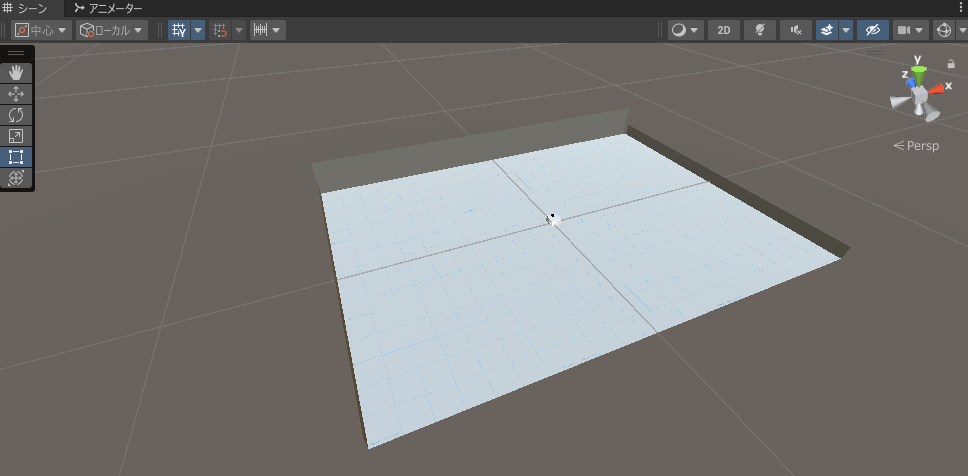
\includegraphics[keepaspectratio, width=0.8\columnwidth]{resources/2024-08-09-mat.png}
  \caption[short]{Matオブジェクトを敷き詰めた図。問題なく走行できる。}
  \label{fig:20240809-mat}
\end{figure}

次回は十分な広さをもたせた空間内でtoioを巡回させられるようにしたい。

カメラ追従、壁、障害物、異常オブジェクトの配置、巡回プログラムの開発。この3つが巡回の残タスク。次回も頑張ろう。

\section*{2024.08.12}
4日ぶりの研究活動。

今日は前回の日記に書いてあった感じで、屋内レイアウトと異常オブジェクトを配置していく。屋内レイアウトは静的オブジェクトか、めちゃ重Rigidbodyでいくとして、異常オブジェクトはどうしようか?

こんな感じでどうだろう

\fboxsep=0pt             %画像と枠線をくっつける.
\fboxrule=1pt            %枠線の太さを1ptにする.
\begin{figure}[h]
  \centering
  \fbox{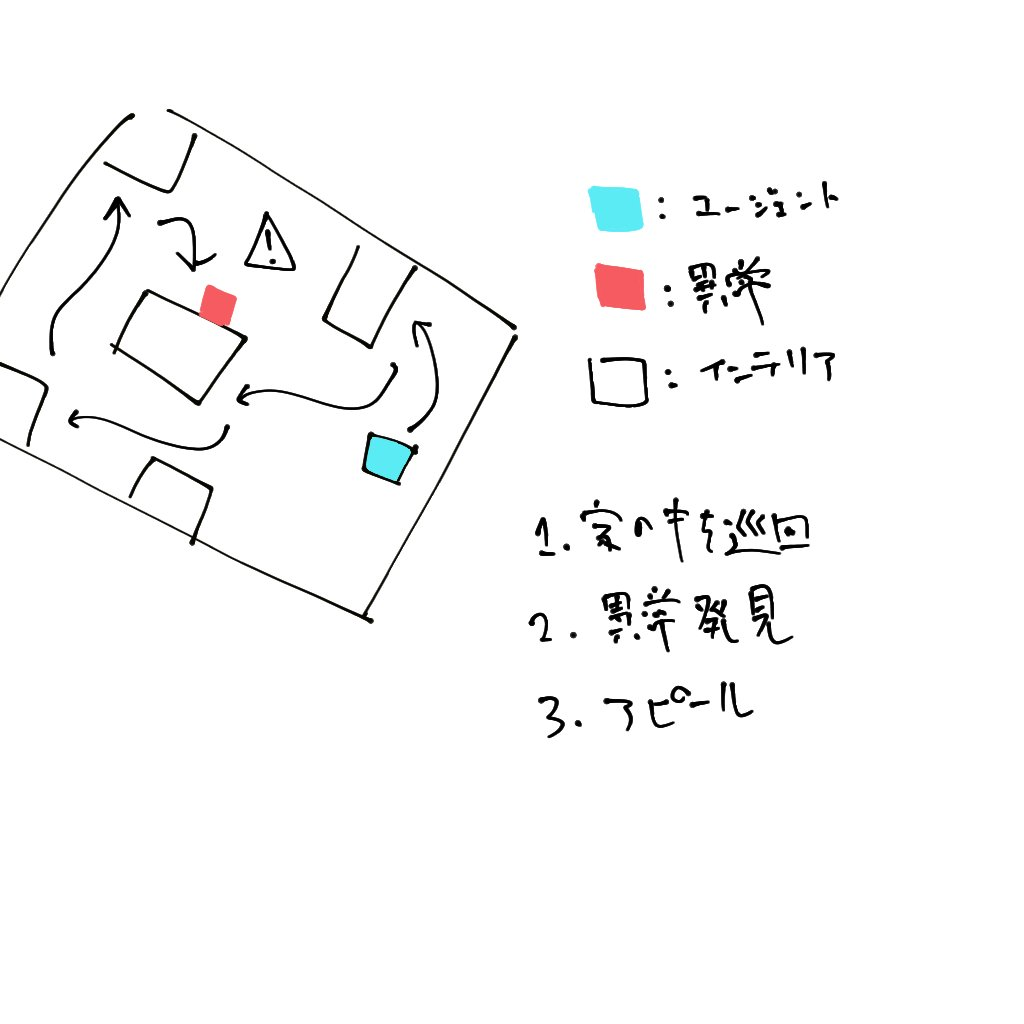
\includegraphics[keepaspectratio, clip, width=0.8\columnwidth]{resources/interior-sketch.jpg}}
  \caption{内装モデルのスケッチ}
  \label{fig:interior-sketch}
\end{figure}

異常オブジェクトはUnity内だけならCollisionイベントで行けそう。じゃ、やってみよう。

衝突部分はできた。問題の巡回部分をアレコレ調べてた。

とりあえずまったく方針がわかないのでClaude様に聞いてみたら、なんかすごくいい感じのプログラムを教えてくれた。動かしてみた結果が図\ref{fig:patrol-draft}。

\fboxsep=0pt            %画像と枠線をくっつける.
\fboxrule=1pt            %枠線の太さを1ptにする.
\begin{figure}[h]
  \centering
  \fbox{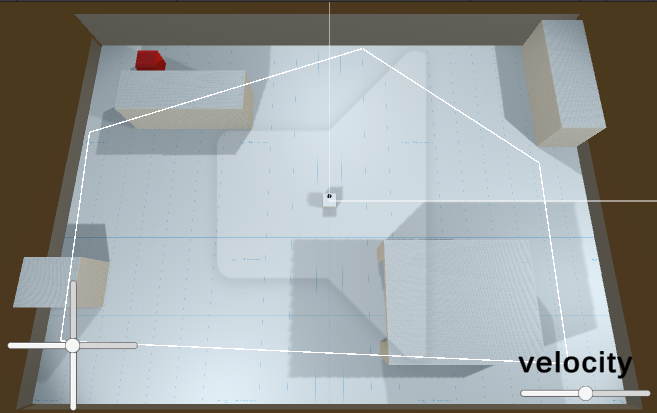
\includegraphics[keepaspectratio, clip, width=0.8\columnwidth]{resources/patrol-draft.png}}
  \caption{Claude様に実装していただいた巡回プログラム。}
  \label{fig:patrol-draft}
\end{figure}

ちょっと見えにくいけど、内装の各地点を結んだ五角形ができてる。これにしたがってtoioが動くようになってる。

ただし現状ではtransformをじかにいじくったようなきっしょい動きになっているので、ここからtoioを動かすプログラムとして書き直す。とはいえこのレベルでイメージを掴ませてくれたClaude様は本当に頭が上がらない。お金払おっかな……

\subsection*{方針1: MoveToで動かす}
toio-sdkにはMoveToっていう機能があった覚えがある。座標を決めて、「ここに行ってください」っていうのを使う。巡回ルートのイメージは、Claude様からもらったプログラムで掴んだし、似たようなことをすればいいと思う。懸念はMoveToを現実空間でも使えるかどうか。なんかマットの上だけだった覚えがするんだよなー……

\subsection*{title方針2: TargetPoleを使う}
Unity限定機能「ターゲットポール」。これを使うとターゲットポールに向けて緩やかに走行させることができる。エージェントごとに巡回ルートとしてターゲットポールの座標を渡しておいて、タゲポ1についたら1を削除、2のインスタンスを生成……みたいにできないだろうか。

Unity上での巡回シミュレーションは作れる目処が立ってきた。今後残りそうな課題はこれをどうやって現実空間で利用していくか。

いま一番行けそうな方法は、エージェントのセンシング昨日で空間情報を把握して、それを管理システムに送る。そして管理システム上で仮想の屋内空間を生成して、その中でMoveToを使えるようにする。みたいな実装だろうか。

ともあれマット上とはいえど巡回ルートが作れそうだから、そのやり方で一旦形にしてみよう。

\subsection*{あとやること}
\begin{itemize}
  \item readmeにtodoリストをつける
  \item 巡回プログラムtoio版の実装
\end{itemize}

巡回できるようになったら、異常発見とかアピールとかの弱さの部分に移っていこう。更にいうとセンシングもどうするかまだ分かってないしな……

\section*{2024.08.16}
toioの巡回システムをつくる。今日は巡回の動き部分。ドキュメント読んで確定したのは、toio.Move関数じゃなくて、CubeHandle.Moveを使いましょうということ。CubeHandle.Moveはモーターの挙動とかの低レイヤーの動きを考えなくていいようなので、こっちのほうが考えたいことだけ考えることができる。音鳴らしとかLチカはまだ低レイヤーな気がするので、こっち側で関数を作ろう。

えーっとCubeHnadleを使ってCubeを動かすためにはまずCubeManagerで繋がないといけなくって……

\subsection*{企画の再確認}
かなりためになるインディーエロゲ開発者ニキの話を聞き、企画書が大事だと感じたので、自分の研究企画について再確認する。
\begin{description}
  \item[企画名]\mbox{}\\
    ちっちゃくてかわいい家政ロボットで、生活を助けてもらう
  \item[コンセプト]\mbox{}\\
    小さくてカワイイキャラに生活を助けてもらいたい
  \item[ジャンル]\mbox{}\\
    ロボット、マイコン、IoT、ちびキャラ、マスコット
  \item[計画]\mbox{}
    \begin{itemize}
      \item[8月: ]Unity上でプロトタイプ
      \item[9月: ]現実でプロトタイプ
      \item[10月: ]Unity上で機能拡張
      \item[11月: ]現実で機能拡張
      \item[12月: ]実戦投入、データ収集
      \item[翌年1月: ]資料整理、発表
    \end{itemize}
  \item[売れそう?]\mbox{}\\
    かわいさ、ちんまりさ、いい意味でのダメさをうまく出せば売れる
  \item[効果測定]\mbox{}
    \begin{itemize}
      \item 生活環境の場所ごとの改善タスクの実行回数が有意に増えるかどうか
      \item ロボットの魅力、すなわち「弱さ」が伝わっているか
      \item 「弱さ」が改善タスクの増加に寄与できているか
    \end{itemize}
\end{description}

企画としては面白そう、というか頭のおかしい企画ではない。実現可能性については、計画の見積り不足がどれくらいかによる。それぞれのステップが実際にどれだけあるか分からないのと、おれの自制力が問題。自制力をアテにしている時点で駄目になりそうな感があるところが怖い。どちらかというと働き方改革?しかしながら見積りミスがおきた時点でどこをカットして次に進むかを考えないと後に後に詰めていくことは想像に固くない。PMの学びを活かせ。

\section*{2024.08.17}
move2系のステップどんな感じだ?まずはシンプルに座標入れて1回だけmove2。次に外から座標渡して1回move2。次に複数座標渡して順番にmove2。うん、この3ステップだな。

\section*{2024.08.27(火)}
LoLばっかりやってるわけにもいかないので、10日ぶりに研究を再開。

目下の課題は衝突検知が機能しないこと。Unity上ならColliderのCollisionイベントで衝突検知はできるんだが、現実ではそんなもの存在しないので、toio備え付けの衝突センサで検知できるようにしたい。

サンプルコードをコピペしたもののうまいこと機能してくれない。

\subsection*{現実での衝突移動できた}
でぎだ!

\begin{itemize}
  \item \href{https://www.youtube.com/watch?v=-0CJAu6-GsE}{toio巡回の現実世界での実装}
\end{itemize}

こまいdiffはgit見ればわかるだろうけど、とりあえずAutoPatrolのプログラムを修正して、サンプルと同じ内容になるようにした。接続部分はCubeManager版だからそっちを見たけど。

\begin{itemize}
  \item \href{https://morikatron.github.io/toio-sdk-for-unity/docs/tutorials_basic.html#9-cubemanager\%E3\%82\%AF\%E3\%83\%A9\%E3\%82\%B9\%E3\%82\%92\%E7\%94\%A8\%E3\%81\%84\%E3\%81\%9F\%E3\%82\%BD\%E3\%83\%BC\%E3\%82\%B9\%E3\%82\%B3\%E3\%83\%BC\%E3\%83\%89\%E3\%81\%AE\%E7\%B0\%A1\%E7\%95\%A5\%E5\%8C\%96}{CubeManagerを用いたtoioへの接続}
  \item \href{https://toio.github.io/toio-spec/docs/ble_sensor/}{衝突センサ周りの技術仕様}
\end{itemize}

まだ検知が不安定なので、もっと衝突検知のシステムを深ぼるか、別の検知機能で補うかしたいな。明日ゼミ行ったときにtoioばらまいて動かしてみるか。

\section*{2024.09.09(月)}
お久しぶりです。やること整理する。

\fboxsep=0pt            %画像と枠線をくっつける.
\fboxrule=1pt            %枠線の太さを1ptにする.
\begin{figure}[h]
  \centering
  \fbox{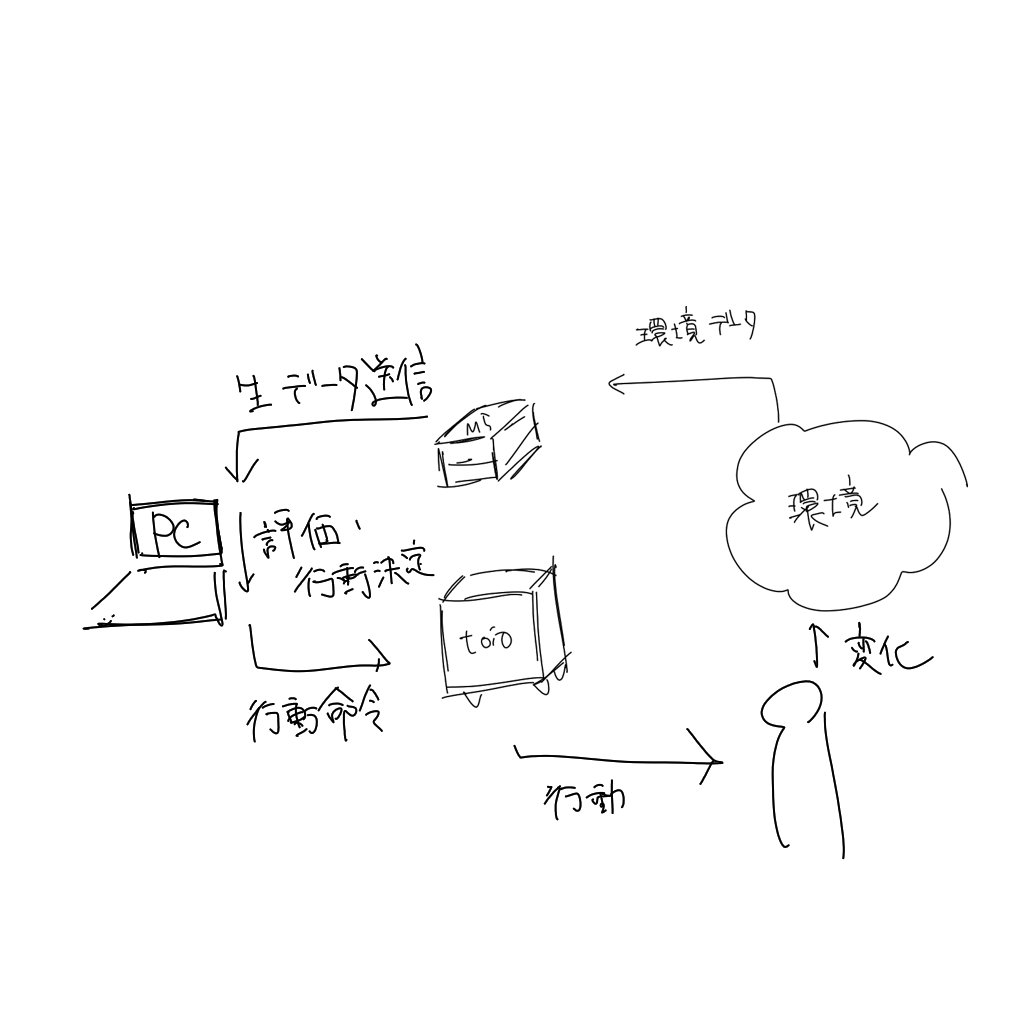
\includegraphics[keepaspectratio, clip, width=0.8\columnwidth]{resources/weak-toio-system-flow.jpg}}
  \caption{本システムのフロー}
  \label{fig:weak-toio-system-flow}
\end{figure}

システム全体の構成は図\ref*{fig:weak-toio-system-flow}のようになる。

現状はtoioの行動部分だけを作った。

次はセンシングして弱い行動の部分。センシングはM5Stickで、行動はtoioで行う。まずはセンシングから。

M5Stickって何を検知できるんだっけ?

\begin{description}
  \item[M5StickC本体]\mbox{}\\
    加速度、ジャイロ
  \item[ENV.2]\mbox{}\\
    温度・湿度・気圧
  \item[ToF HAT]\mbox{}\\
    距離
\end{description}

んじゃあ気温系はENV使わないと無理だな。やってみよう

\begin{itemize}
  \item \href{https://qiita.com/visyeii/items/e28f8500f43166710664}{M5StickC PlusでENV II (環境センサユニット)を動作させる}
\end{itemize}

本家に入っていたENVのサンプルスケッチが動かなかったので、こっちの記事にあったコードを使用。動いた。

\section*{2024.09.18(水)}
M5にENV2取り付けて気温データ取得するところまで組みたい。なんだか周りの人間もだんだん動き出して来てるっぽい。もっとやすんでていいんだよ

BLEを使って通信できないかと調べてみたけど、難しそうなので一旦普通のBluetoothシリアル通信で実装する。

\section*{2024.09.19(木)}
エラー集を充実させたい。

今日の進捗はなかなかだぞ。お昼いっぱいやってただけあるな。M5StickCとENVのデータ取得とシリアル通信での送信を実装した。ChatGPTを使ったらほんとすごい進捗あがる。その上動くコード完成させるだけじゃなくて、クラス化したりファイル分けしたりで構成もだいぶきれいにできた。まじでおもろい。次回はUnity側での受け取りをしたいから、Arduino側のprintf側でUnity用の区切り文字追加するのと、Unity側でのBluetoothシリアル通信の実装。このへんは昔取った杵柄って感じで、スムーズに行ってくれるとラクできるんだけどなあ。

\section*{2024.09.23(月)}
M5StkckCからUnityにシリアル通信でデータを送る。のだが、なぜか配列外参照エラーで止まる。今日はもう酔って作業どころではないので、寝て明日やる。

\section*{2024.09.24(火)}
昨日クソ眠くてできなかったシリアルデータの送信を実装。

なんでできてないんだろと思ったらimuInfo側の配列参照をミスってた。6個しかスロット無いのに7番目にアクセスしようとしてた。

めちゃくちゃ便利だったのが下の2つ。

\begin{lstlisting}[caption=Unityのエラー表示,label=code:error-output]
// 具体的にどこでエラーが起きたのかを表示
Debug.LogError(e.StackTrace);
\end{lstlisting}

前に佐藤先生がブレークポイント使うといいよって言ってたのに加えて、こういうエラー表示系の機能についても勉強しておくと、エラー処理がめっちゃ簡単になると思う。まああとはChatGPTな。あいつまじで便利。

今日はM5StickCからUnityへのデータ送信を実装した。次回は評価リストと行動リストをつくる。可能なら「評価」の部分も実装できると偉い。

\section*{2024.09.26(木)}
このロボットが一番映えるシーンやシチュエーションを考えて、それを解決できるような特殊実装を目指してみたらいいんじゃないって言われたので、シチュエーションを考える。

基本的には気温取得系は向いてるっぽい。となると換気系のシナリオ。

\subsubsection*{2台のロボットで換気行動を誘発}
2台の異なる役割を持ったロボットが存在する。
\begin{description}
  \item[1台目:]環境情報を取得するロボット
  \item[2台目:]人間に呼びかけを行うロボット
\end{description}

環境情報を取得するロボットは、リビングとかに置く。

呼びかけるロボットはユーザがいる部屋に置く。

環境機が今いる場所の気温湿度が不快になったら、環境機から呼びかけ機に通信。呼びかけ機がユーザに向けてアラートを出す。

ユーザは呼びかけに気づいて、リビングの方に行く。環境機が不快を訴えたり、リビングが不快であることに気づいてエアコンつけるなり窓開けるなりする。

人間がその場にいるならその場でアラート出せばいいけど、ロボットを置いておくことで、少し離れた場所でも監視が可能になる。

テレワークや介護、子供の世話とかしてる方に便利そう。

\section*{2024.10.01(火)}
弱くて小さいロボットが役に立つシーンを考える。

ベースは環境データの取得と遠隔での呼びかけ。通知もシステマチックなものじゃなくて、ロボットが動いたり鳴いたりすることで呼びかける。
\subsubsection*{お年寄りの介護}
自分の親を介護しながら在宅で仕事してる人。介護のときは当然同じ空間にいるけど、仕事や自分の時間のときはそれぞれ違う部屋にいる。

そういうときに、自分の部屋には呼びかけ機、親の部屋にはデータ取得機を置く。これによって離れていても何かあれば通知してくれるので安心。

カメラはつけない。監視してるみたいだし。そういうんじゃないと思う。お互いの様子を見れて、かつ、何か合ったときに教えてくれるペットがいるような感じにしたい。

データ取得機は、おじいちゃんおばあちゃんの部屋で環境データを取得し続ける。その間に、室温が高すぎるとか、じめじめしてるとかになったら鳴きだして警告する。おじいちゃん達が自分で動けるならこの時点で自分等でエアコンつけたり換気してもらってもいい。もしそういうのも難しいのであれば、ここで呼びかけ機に通信して、仕事してる若い人に通知して、様子を見に来てもらう。そしてエアコンつけたりして環境を整えてもらう。

主な利点としては、自分でいちいち気温を気にしなくていいところ。ロボットがつねに確認してくれるので、調整が必要になれば言ってくれる。何かあれば呼ぶので、ロボットを置いておくだけで、おじいちゃんたちに気負うこと無く、自分の作業をこなすことができる。おじいちゃんたちを監視する機械を設置するのではなく、何かあったときに介護の人を読んでくれるペットを置くようなイメージなので、介護される側も窮屈に感じない。また置くだけなので場所に制約されない。介護の人と介護される人がいる部屋それぞれに置けばいいだけ。

\section*{2024.10.02(水)}
今日は機能をつくります。なんの機能?環境データ関連の機能。あとダミーデータ生成機も作りたい。

\section*{2024.10.05(土)}
評価システムの設計をした。ChatGPTと相談の末、結構安心して作れそうな設計と実装例ができたので、次回はこれを実装していきたい。

やる前の適当な予想だけど、評価ロジックと実際の挙動の実装が多分一番面倒くさい。多分マジで面倒臭いからその辺うまいことChatGPTに投げつつ作ろうかな。

あと設計の過程でUML作ったよ。tasklogと同じ階層に置いたはずだからちょくちょく見てね。

\section*{2024.10.07(月)}
テストがしたいのでUnity Test Runner を使おうとしたけど、テストがうまくできなかった。でもできるようになったら自作クラスの単体テストとか効率的にできそうなので、やりかたは覚えたい。

toio-sdkのテストか何かが噛んでるっぽいのでそれを解決したら治るんじゃないですかね。邪魔やねん。もうダルいので今日は絵を描く。

\section*{2024.10.08(火)}
今日はUnity Test Runnerの使い方を覚えたい。

動かせるところまではいった。エラーは直らない。

テストが上手くいかないのはtoio-sdkのせいではないということは分かったのでそれで許す。おれが悪いよ。

次回はテストやってエラー解決方法見つけたりなんだりできるところまでいくとうれしい。

\section*{2024.10.10(木)}
今日もシステム作ってた。対象とする環境データを指定しながら、その上で評価クラスと行動決定クラスを自動で決める構造が作れないかやってたけど、上手くいかないのでくっそシンプルに作り直した。なんかよさそう。ChatGPTもいいんじゃねって言ってくたし。

\fboxsep=0pt            %画像と枠線をくっつける.
\fboxrule=1pt            %枠線の太さを1ptにする.
\begin{figure}[h]
  \centering
  \fbox{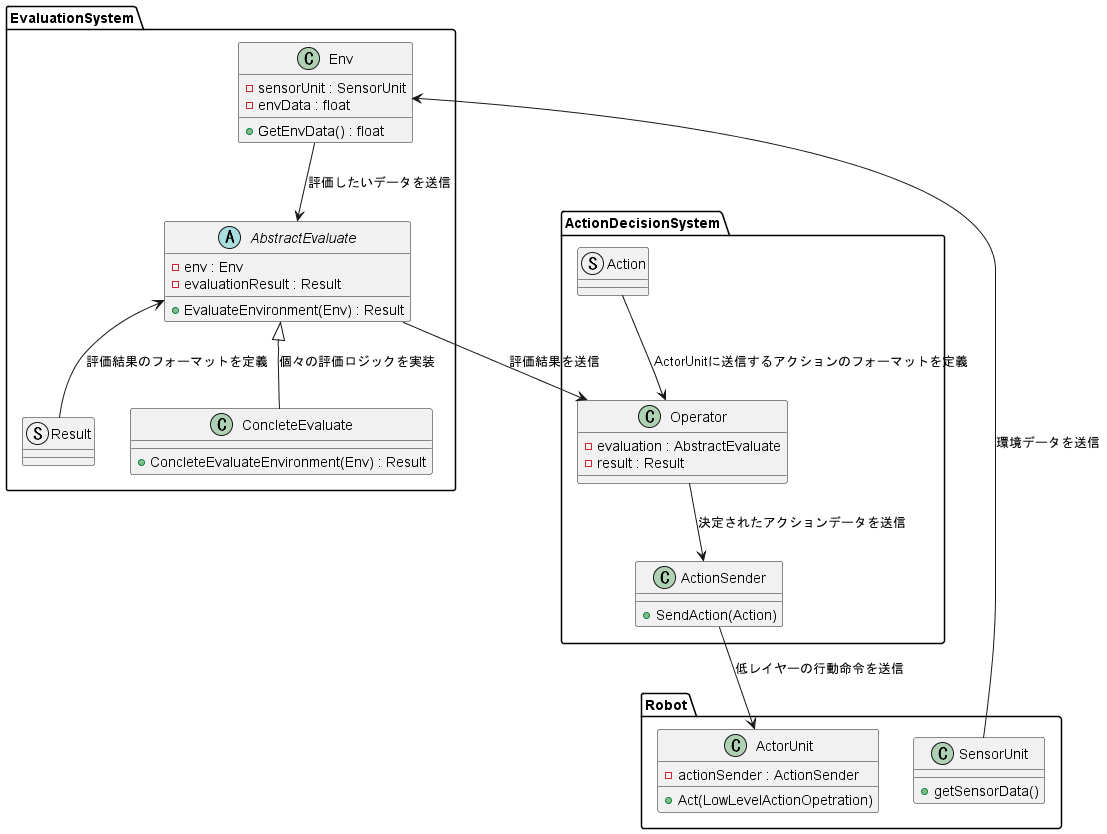
\includegraphics[keepaspectratio, clip, width=0.8\columnwidth]{resources/evaluate_environment.png}}
  \caption{}
  \label{fig:}
\end{figure}

\section*{2024.10.12(土)}
この前一応完成した設計を実装する。実装する途中で色々困ることになるとは思うが、適宜解決しつつ進めていきたい。

\fboxsep=0pt            %画像と枠線をくっつける.
\fboxrule=1pt            %枠線の太さを1ptにする.
\begin{figure}[h]
  \centering
  \fbox{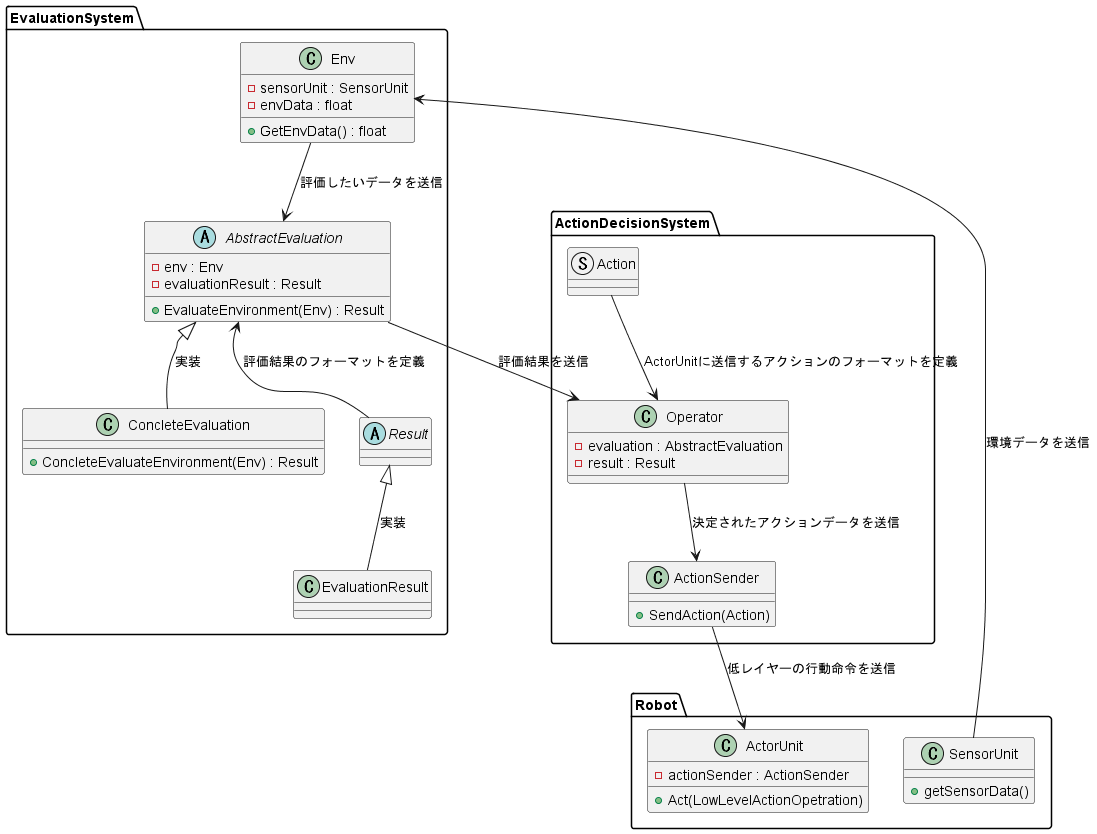
\includegraphics[keepaspectratio, clip, width=0.8\columnwidth]{resources/evaluate_environment_2.png}}
  \caption{評価システムの設計 第2版}
  \label{fig:evaluate-environment-2}
\end{figure}

設計はできたから、あとはどうしたら評価ができるか。

現在の気温、もちろん要る。基準となる気温、これはどこから取ってくる?気象庁とか、オフィスワークにめっちゃ詳しい団体が情報を公開してくれていると助かる。閾値、これは基準となる気温からどれくらい離れているかを測る。「暑い」「寒い」「快適」の3つがいいだろう。

初めて自作クラスのテスト通るところまでいけた!結構嬉しい。

toio-sdkの問題か分からないけど、Editor起動して一番はじめのテストはPlayModeでtoio-sdkのテストを実行しないとテストがちゃんと動かなくなるっぽい。通るテストできたし、今度検証してみよう。

Unityでスクリプトつくるうえで結構大事そうなことも分かった。すなわち、「Monobehaviorの継承はUnityと連結したいスクリプトだけ行う」ということ。

多分オブジェクト指向とかが多少わからないとそもそも継承とかを使わないので中級者向けの考え方ではあると思うけど、自作クラスは無継承で作って、Unity上に配置するところに自作クラスとゲームオブジェクトをつなぐMonobehavior継承クラスを挟む。まさにインタフェース。

多少調整は必要だけど、Unity上で100\%オブジェクト指向設計ができるようになるこの作り方は絶対必要になると思う。

デバッグ用につくってるダミーデータ生成器のデバッグ表示機能がおかしいので、次回はそこを修正しながら、EvalutionSystem全体のテストとか、さらにActionDecisionSystemの実装も進めていきたい。

\section*{2024.10.16(水)}
エラー表示は機能なんとかしました。ログ書き忘れてたけど、前回(15日?)の研究でエラー表示直して、エラー判定とかせずに挙動確認するだけのテスト作った。

今日はActionDecisionSystemの開発に着手しだした。ActionがResultによるということで、Result側で抽象を完全に切ってしまう必要が生じた。いまActionもAbstractで組もうとしてたけど、そんな密結合のクラスやめたほうがいいって。Resultで切れるなら切ったほうがいい。

というわけで、次回はActionに渡すResultのフォーマットを決めて、Resultの具象クラスでそのフォーマットで全部渡すように組み直して、みたいな作業を進めていければと思います。

\section*{2024.10.17(木)}
今日からはActionDecisionSystemをメインに作っていく。

のだけれど、その前にResultをActionDecisionSystemに渡す部分について考えなければいけない。具体的には、Resultのフォーマットを制限せずにActionDecisionSystemに渡すのか、Resultのインタフェースを定めて、ActionDecisionSystem側からシンプルにアクセスできるようにするのか。

でもそういう2項対立だったら、ポリモーフィズムできるんだから絶対にインタフェースを定める方式にしたほうがいい。

となると問題になるのは、Actionを決めるために、Resultに何があれば十分か、ということ。かつResultインタフェースが持つものは、個々の対象に依存した概念ではなく、Result一般が持ちうるものである。

パット思いつくのは、はじめにCondition。これは絶対にいる。でも、現状のConditionの形だとデータの内容がばらつき過ぎて駄目だ。気温はHOT,COLD,SUITABLEだとして、じゃあごみがあったり湿度が高かったりしたときも同じようにできるわけじゃない。共通化するか、括り方が間違っているか。なんとなく括り方が間違っている気がする。評価とそこから派生する行動は切り離せないのでは?正確には評価と派生する行動の基準のようなもの。暑いときに寒いときやゴミがあるときの行動は取らない。のであれば、やっぱり環境評価と行動決定は密結合でいい。

これや!
\fboxsep=0pt            %画像と枠線をくっつける.
\fboxrule=1pt            %枠線の太さを1ptにする.
\begin{figure}[h]
  \centering
  \fbox{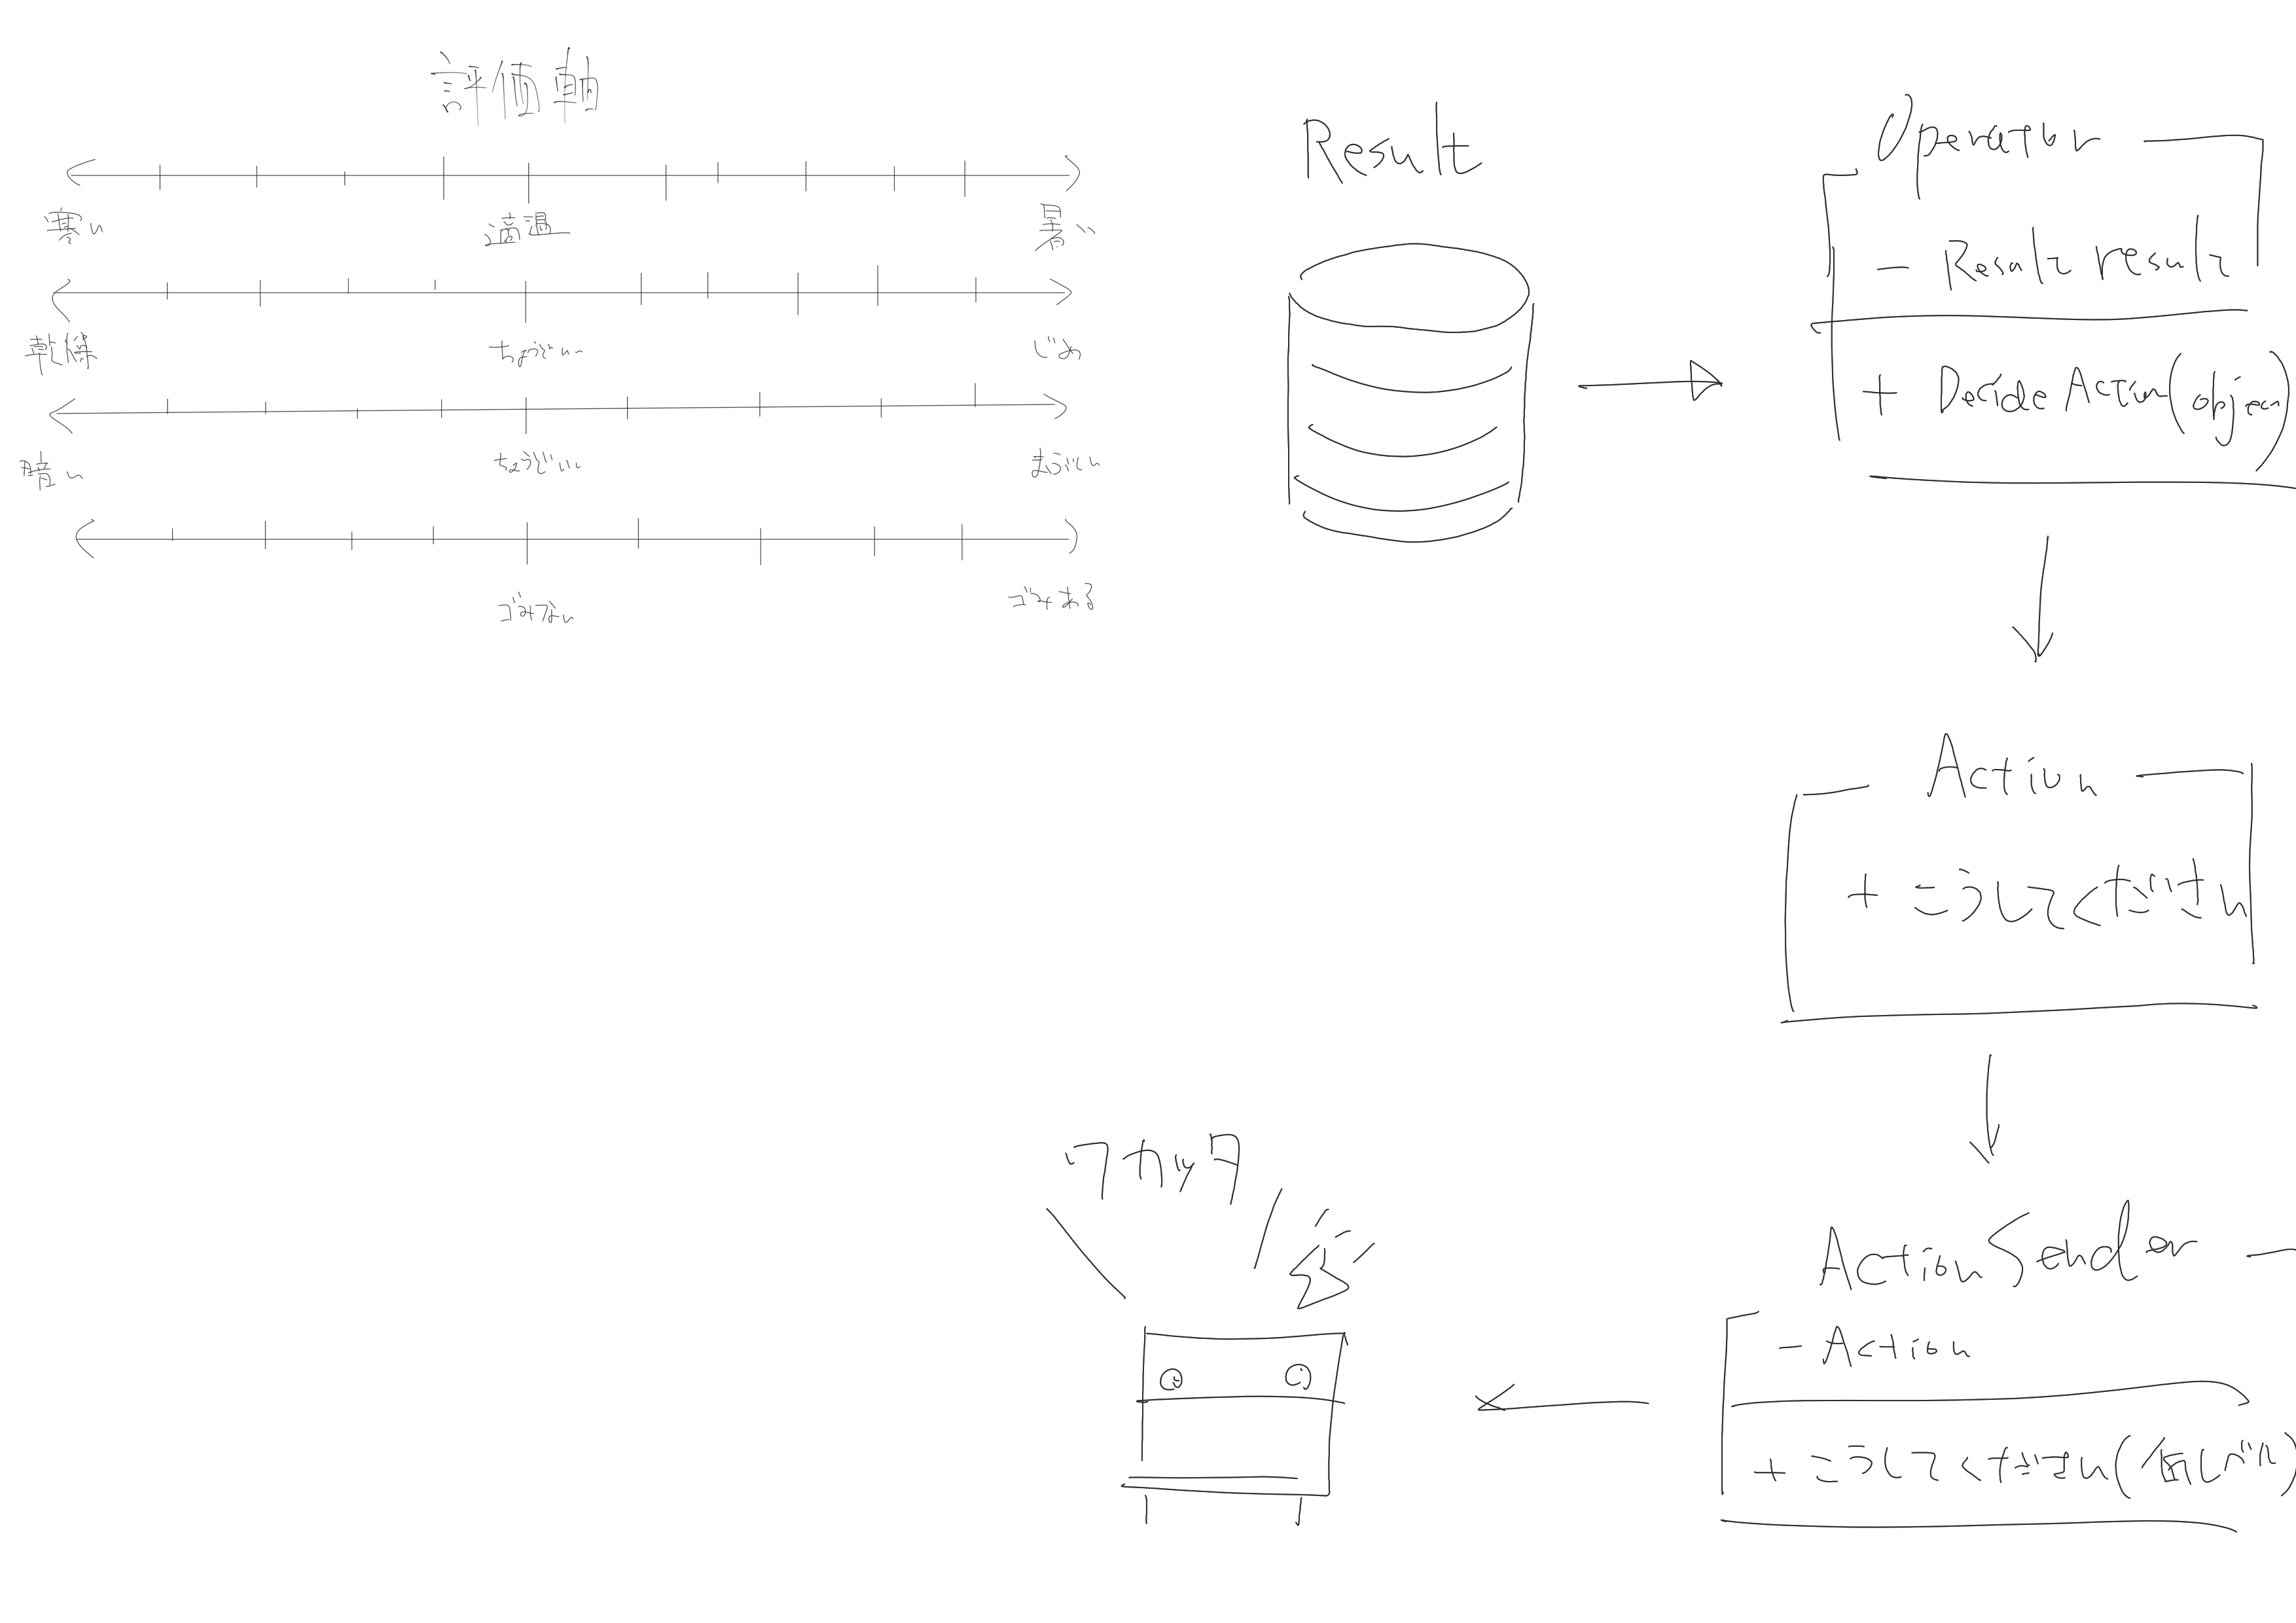
\includegraphics[keepaspectratio, clip, width=0.8\columnwidth]{resources/20241017_ActionDecisionSystem_sketch.png}}
  \caption{評価データの扱いおよびResultのフォーマット、それをどうAction以降に送るか}
  \label{fig:EcaluateFormat}
\end{figure}

今日はサンワ棚をお迎えするために終わる。

次回はResultに入れるデータフォーマットおよびそれを入れる部分の作り直し。設計の修正。あといろいろやっておいてくれ。

\section*{2024.10.21(月)}
Resultの内容を前回決まった数値判定式に変えた。\href{https://www.mhlw.go.jp/content/11300000/000905329.pdf}{厚生省}のドキュメントによると18℃~28℃が適温らしいから、その範囲に従って採点するように作り変えた。次回はDummyDataGeneratorと合わせて採点が動くところまで確認した

\section*{2024.10.22(火)}
ダミーデータを生成してEvaluationで評価する部分を作った。コルーチンの使い方もなんとなく覚えた。問題なく数値は流れていたので、次回はActionの決定部分を作っていく。

\section*{2024.10.23(水)}
データ渡す部分ができたので、行動決定の部分を作っていく。いまの構想としては点数化したResultをActionOperatorに渡し、点数にしたがってアクションを決める。非常に単純。

ダミーデータでの挙動チェックは前回やったが、実際のセンサーユニットを使った挙動チェックはやっていなかったので、そこもやっておきたい。チェックが終わったら行動決定をの設計をする。時間があれば実装まで着手。

SensorUnitがアタッチできない。なので付け替え実装というより、M5とダミーのメインループを行うコンポーネントを作って、都度アクティブにするような運用。

SerialHundlerをオブジェクト指向に取り込むためには、SerialHundlerをシングルトンにする。んでもってUnityのシステムを一切使わせないようにする。関数はそのまま、SerialHundlerを使うスクリプトで呼び出させる。んでもって、COMポートとかボーレートはエディタで設定できた方が便利だから、ScriptableObjectかMonobehaviorとしてつくる。

センサー部分をポリモーフィズム使用としたら思ったより難しくて中断。でも設計はしたので、面倒だけど次回からやっていく。
設計は図\ref{fig:serial-config}の通り。

\fboxsep=0pt            %画像と枠線をくっつける.
\fboxrule=1pt            %枠線の太さを1ptにする.
\begin{figure}[h]
  \centering
  \fbox{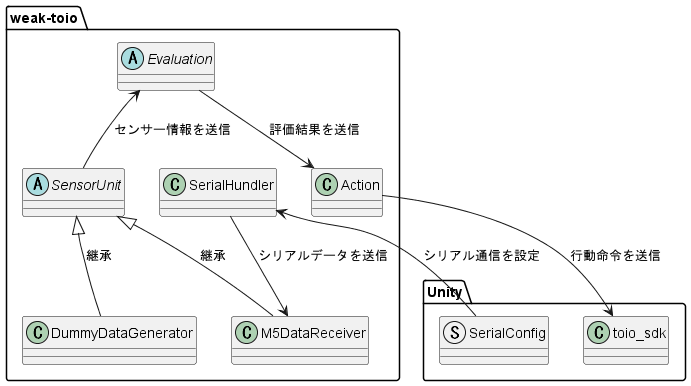
\includegraphics[keepaspectratio, clip, width=0.8\columnwidth]{resources/20241023_SerialConfig.png}}
  \caption{}
  \label{fig:serial-config}
\end{figure}

\section*{2024.10.27(日)}
センサーとダミーデータを使い分けられる構造に作り変えて、センサーからの情報がちゃんと届いてることが確認できた。

でもおれの体幹よりも気温高めだったので、センサーとは相性が悪いかもしれない。

気温データは適温の範囲から外れるほど、正負のどちらかに傾くスコアを持たせたので、アクション決定ではこれを利用してアクションの強度や種類を決めるようにしたい。Acstractでつくるのは大変なので、とりあえず気温から汚く作っていく。

アクションのアイデアを図\ref{fig:weak-toio-action}に示す。

\fboxsep=0pt            %画像と枠線をくっつける.
\fboxrule=1pt            %枠線の太さを1ptにする.
\begin{figure}[h]
  \centering
  \fbox{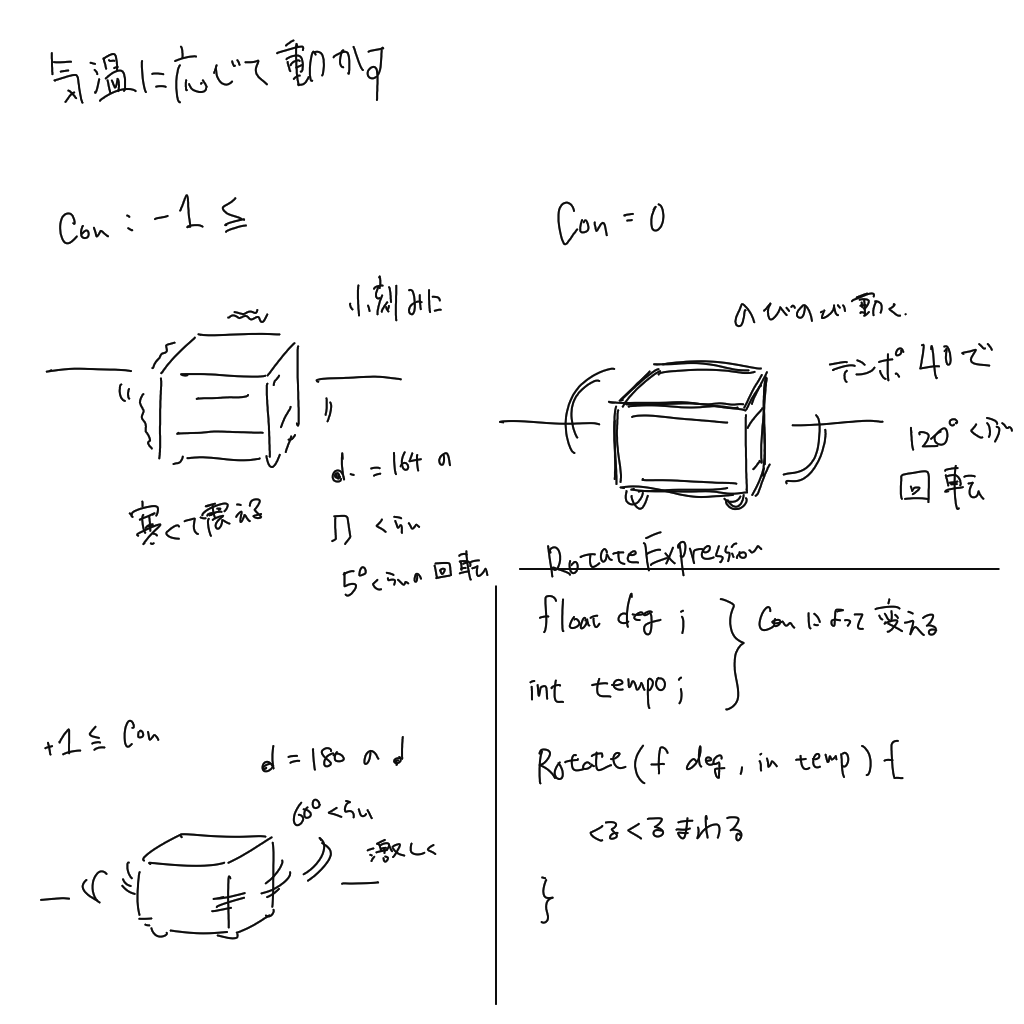
\includegraphics[keepaspectratio, clip, width=0.8\columnwidth]{resources/20241027_weak-toio_1.png}}
  \caption{}
  \label{fig:weak-toio-action}
\end{figure}

パラメータは「角度」と「回転のテンポ」の2つ。

うん、すっげえ汚えけど、きれいな設計思いつかないから後で考えよう。

それはそうとアクションのデータフォーマットはどうする。Resultで入手できるのはスコア。じゃスコア。あとロボットのアクションの強度を決めるのに必要なパラメータ。

そういえば最終的にシステムとして動かす場合、メインループは1つでいい。並列処理とかしないなら。なのでMonobehavior系のスクリプトは1つあればよい。ほかは基本的にUnityが無くても動くように調整できてるはずだし。

そっち側のメインループスクリプトをものっっっっそい荒いけど書いてみた。多分こういう風に動いてくれるよねっていう10割イメージで。

明日はAutoPatrolあたりを見返して、ロボット動かすメソッドと、コンディションに応じてメソッドを自動で選択する方法を考える。先に寒い・適温・暑いの3パターンの関数を作ってから考える方が時間のムダが無くていいでしょう。

\section*{2024.10.28(月)}

\begin{alignat*}{2}
  & 付点四分 = 164 \\
  & 八分 = 552 \\
  & 四分 &&= 276 \, [\text{bpm}] \\
  & &&= \frac{276}{60} \, [\text{bps}] \\
  & &&= 4.6 \, [\text{bps}] \\
  & 1\text{回回るのに必要な時間は} \\
  & 1 \, [\text{s}] / 4.6 \, [\text{bps}] = 0.217[\text{秒}]
\end{alignat*}

メインループで動かしてみた。んだけど、これといって何も動かない。toioが無いから?でもデバッグ表示ではM5もちゃんと動いてるみたいだし、評価もできてるよう。次回ダミーデータ版のメインループつくりつつ、toio動くところまで確認できないかな。

\section*{2024.10.30(水)}
RotateByDeg 系の関数は RotateSpeed > 15 のときのみ機能する。

全く思いつかない。キャラ追加みたいにモーション追加がしたいけど、モーションデータの扱いがわからない。Json?モーションのデータセットを別で持って、その中身をシステムが全部読みこむ感じ?じゃあ Json の Read がいるじゃないですか。

震えるモーションを作っただけではだめなので、今の時点で拡張性を持たせなければならない。理想を言えばモーションはリストみたいに所持できて、必要に応じて任意のモーションを選んで実行するようにしたい。

モーションをキューで管理する。イベントに応じて対応するモーションクラスを拡張した具象モーションインスタンスを生成して、モーション実行クラスのキューに追加する。

モーションクラスは任意のモーションおよびその時間を持っていて、モーション実行クラスはモーションインスタンスに入っているモーションを時間分実行する。実行されたモーションはpopされ、次のモーションクラスが実行される。

\section*{2024.10.31(木)}
全然設計が思いつかないので、今考えていることを書きなぐる。

システム全体は4つのパッケージで構成される。

\begin{enumerate}
  \item エージェント部: ロボットおよびセンサーユニットを制御
  \item 評価部: センサー情報を取得して環境を評価
  \item 行動発行部: 評価結果をもとに行動命令を発行
  \item 行動実行部: 発行された行動命令を逐次処理
\end{enumerate}

エージェント、評価は完成していて、行動実行もイメージは湧いてる。行動発行部の設計が思いつかない。

こういうときは逆に、評価部から出せるものと、行動実行部が欲しいものを先に決めればいい。入口出口が決まっているなら通路も比較的決めやすい。

評価部で新しく追加されるデータは環境の「評価スコア」。現状は正負どちらにも傾きすぎればよくないとして、0を適正値としてスコアを返す。その他センサー情報もセンサーユニットから送られたものはそのまま流すことができる。

行動実行部では、送られてきた行動命令を逐次実行する。そのため、toio-sdk用の行動命令のキューがほしい。キューをpopで処理していけば、逐次実行は実装可能だと思う。実行はUpdateじゃなくてコルーチンにすれば命令のオーバーフローも抑えられると思う。

では具体的にどのような行動命令であれば、上のことが実現できるか?

まず考えられるのは、行動の具体的なパラメータ。toio-sdkではマットを使用しないアクションとして、前後に移動するTranslate、向きを変えるRotateByDeg/Rad、その他音を鳴らしたりLEDをつけたりさせることができる。

となると、させたい行動のタイプによって必要なパラメータが異なるので、各行動用の構造体が必要になる、また行動のタイプを決定するために、行動タイプをまとめたenumも必要になる。

MotionOperatorで行動を実行するから、MotionGeneratorではモーションのレシピを発行するようなイメージ。接客して、欲しいもの聞いて、それをキッチンに連絡する。

明細発行、というと、なんだか昔似たようなクラス設計を目にした気がする……

ひとまず今日は時間になったのでここで終わる。次回も書き殴りから初めて、必要なものを整理していこう。

\subsection*{行動実行部でいるもの}
\begin{itemize}
  \item 行動タイプ: enum
  \item 行動パラメータ: タイプによって異なるパラメータ
\end{itemize}

\section*{2024.11.01(金)}

行動タイプはevaluateが発行して、resultを通して渡す。

行動パラメータは、行動タイプに応じて、対応する構造体を生成して、その中のフィールドをいじくることで変化させる。パラメータ変化にはresultのscoreを用いる。

行動タイプとパラメータ構造体は1対1で対応付けられている。

行動決定部では、対象とする環境データごとに区切りを決めて、区切りごとのモーションを発行する。

TAやってたら「概要設計」っていう話が出てきた。システムの振る舞いを関数、クラス、コンポーネント単位で記述する。仕様に書いたことを実装するべきだし、仕様にないことは実装するべきではない。おれのシステムの概要設計ってどうなるだろうか?

\section*{2024.11.18(月)}
前回までは、センサープログラムを修正した。Actionを作っていく。

TemperatureActionにいろいろアクション生成っぽい関数があるので、これを実装していく。

どういうアクションがそれっぽいかな?寒い方は震える。暑い方は?わからないので回転させる。

ベースにCold、Hotそれぞれにアクションの方針があり、Danger圏内になったら露骨にする。

コルーチンがだんだん分かってきた。フェーズ式のモーション実行なんかはコルーチンにすればいける。今日は検証の時間って感じだったので、次回次々回くらいには動きの一つでも実装してみたい。

\section*{2024.11.19(火)}
Movementは他のCubeHandlerから作ったものでも使い回すことができる。

ActionGeneratorから作ったActionをActionSenderに流す。コルーチンを使う場合、ActionGeneratorではIEnumeratorを生成する。SenderではIEnumeratorをStartCoroutineする。

アクション命令送信回りのデータの流れが上手くいっていないので、次回は終端からデータの流れを見直す。これメモ。

\fboxsep=0pt            %画像と枠線をくっつける.
\fboxrule=1pt            %枠線の太さを1ptにする.
\begin{figure}[h]
  \centering
  \fbox{\includegraphics[keepaspectratio, clip, width=0.8\columnwidth]{resources/20241119_memo.JPG}}
  \caption{}
  \label{fig:}
\end{figure}

\section*{2024.11.20(水)}
依存性注入を使うと、アクション生成が上手いことできそう。Claudeに聞いた。アクション生成の関数はCubeHandleを持ってるクラスのインターフェースに宣言させる。実装はインターフェースを継承させたToioあたりのクラスにやらせる。

\section*{2024.11.21(木)}
DIハマって、昨日の夜眠れなくてDI使った設計にしたらめちゃくちゃイカした設計になった。
リファクタリングはともかく、さっそくActionの実装に使おうと思う。

\section*{2024.11.23(土)}
DIでAction部分を設計し直したら結局全部作り直すことになった。作り直しはできたが、asyncとかtaskがよくわからないために初期化でエラーを吐かれる。いったん今日はやめにして、次回toioの接続からインスタンスの登録を安定化する。

\section*{2024.11.27(水)}
今日もつまんなく思われるかと思ったが、意外と会話できた。

身体でわかることを通知したところで「そんなんわかるよ」になるので、身体には分からないことを教えてくれる子にしたほうがいいよねって話。「〇〇の気持ち」シリーズつくれ。

非機能要件の話ばかりしてしまう。機能の話苦手なんかな。機能の話できるようになりたい。

\subsection{〇〇の気持ち}
\begin{itemize}
  \item ねこの気持ち
  \item 草の気持ち
  \item 本の気持ち
  \item  部屋の気持ち
  \item 自分以外の人の気持ち
\end{itemize}

\section*{2024.11.28(木)}
バリエーションを作る前に、キューブの動作方式をHandleからCubeに変えたい。いや、Handleの動きに対する強さはそのままに、Cubeで使える便利な機能も使えるようにしたい。

拡張性も考えると、動作はデリゲートにして、動作の主体になるCube、CubeHandleと動作命令を引数にする。

\begin{lstlisting}[caption=,label=]
Toio.Move(CubeHandle, Movement)
Toio.PlaySound(Cube, SoundOperation)
Toio.LED(Cube, LightOperation)
\end{lstlisting}

修正の方針を固めた?ので、明日は実装していく。今日中に実装できるかと思ったが、まあいい。

\section*{2024.12.01(日)}
複数台接続を実装した。メインループで実装するのはアイデアが出なかったので、toioへの接続をメインループから切り出して、ToioConnectorで得られたtoioのデータをメインループに持っていってもらうようにした。キューが相変わらず役に立って、取得したキューブをDequeueすることでキューブの重複を防げているのは自慢ポイント。

複数台接続を実装したことで、「役割別の接続できるようにしたい」という課題も見つかった。次回は「役割」の概念と、役割別の接続機能を実装したい。

前回の日記でCubeとCubeHandleのいいとこ取りをしたいって話をしたけど、多分それも実装できた。これも多分DIで、Toioの動きをIToioCommandっていうインタフェースに包むことで、「実行」っていう機能を抽象化した。一応気温アクション生成に使ってはいるけど、これといって大きな変化は見られない。多分こいつが加賀焼くのはアクションをデザインしていくフェーズなので、それまではくつろいでいてもらおう。

\section*{2024.12.02(月)}
役割理論を考えた結果、役割の実装はできそう。ただ、現状のインタフェースや抽象クラス、メインループといった基幹系クラスが軒並み「M5StickC+ENV2センサーでデータを取得する」という前提に依存しているという問題が発覚した。このままだと役割機能が実装できないので、根本の実装を変える。
アイデアは相変わらずのインタフェース。  M5とかENVとかを全部インタフェースにする。それに伴って、気温判定をするやつはTemperature、距離判定するやつはToFとか、それぞれのインタフェースを求めるようにする。こういう根本からの作り直しはだんだん頭おかしくなってくるから、じっくり焦らず、着実にやろう。

\section*{2024.12.07(土)}
役割分けを実装した。はじめの懸念どおり、スクリプトをアタッチしても、アタッチしたtoioに正しく接続してくれるわけではない。考えとしては、
\begin{enumerate}
  \item M5認証
  \item 1個ずつ認証
  \item 多分接続の優先度が親機からの距離に関係しているので、近いものから順に
\end{enumerate}

みたいな感じ。どうすっかなー……距離比例だったらM5から接続するのが一番丸い。位置情報とかは持ってないし、データとして使うのも難しそうなので使わない。可能ならM5経由してtoioに接続。そうするとデータの流れが全く変わるんだけどね。

おそらく

M5 -> PC -> 判定 -> アクション生成 -> アクション送信 -> M5 -> アクション命令 -> toio

みたいな導線?

イニシャライズは

PC -> M5 -> toio

Arduinoでtoioを制御してる前例はいくつかあったので、それを参考に組みなおしてみようか

\href{https://note.com/vhideo/n/nff5e2845beb1}{toioをESP32(Arduino環境)で動かす}

\section*{2024.12.09(月)}
接続されているtoioをうまいこと識別する方法が無いか探していたら、「ローカルネーム」という概念を使って、toioヒトツヒトツを制御できることが分かった。これを使えば位置情報とかM5からとか難しいことをせずともtoioを分けて制御できそう。

ただ名前を調べようとあれこれしてみたのだが、何故かtoioのローカルネームが出てこない。公式のテンプレートに戻って試してみても不発。ローカルネームはこっちで設定するものではなくて、toioそれぞれが出荷時点から持っている固有の名前のよう。

借りてからしばらく経っているのでシステムの不具合かと思われる。なので今度のゼミのときに持っていって、toioのアップデートをしようと思う。

\section*{2024.12.12(木)}
基幹システムが完成して、あとはセンサの種類とアクションのバリエーションを増やしたら終わり。

あ、人間が気づきにくいシチュエーションを考えるの忘れてた。そこを考えたらつまんねーセンサーも面白く使えそう。

\subsection*{気温}
自分にとっての暑い・寒いはわかる。

でも、自分以外にとっての暑い・寒いはわからない。ここのセンシングを行い、それを知りたい人間に伝える。

\subsection*{湿度}
人間: 「じめっとしてる」はわかる。でも、基本的に何 \% だろうが問題はない。

湿度が問題になるもの
\begin{itemize}
  \item 電子機器
  \item 漆
  \item 布製品
  \item タンス・クローゼットなどの収納
  \item 食品
\end{itemize}

こういうののセンシングを肩代わりしよう。

\subsection*{気圧}
分かる人とわからない人がいる。おれは分からない派。

気圧で調子が悪くなるのはガチらしい。気圧が鬱に関係あるんじゃないかって言ってる人もいるから、モニタリングしてみる価値はあると思う。

\subsection*{CO2}
「空気がこもってる」はわかる。が、「換気する」という動作が周りの迷惑になるんじゃないかと思ってできない場合はあると思う。そういうときにweak-toioが「換気してくんねーかなー」な動作をして換気を促せるといいと思う。

\subsection*{単におもしろそうなネタ}
\begin{itemize}
  \item 店番(対物センサ)
  \item ネコのおもちゃ(?)
  \item 回線速度バロメータ(wifi + cmd.ping or api)
  \item 天気予報(wifi + api)
  \item アラーム、チャイム
  \item 眠気バロメータ
  \item 掃除したほうがいいかどうか
  \item マーチングバンド
  \item 人が来たら演奏するバンド
\end{itemize}

音楽をやろう。全然weakと関係ないけど、楽しそう。

toioで音楽といえば「ピコトンズ」。明日触りに行こう。

あとはwifi接続の方法とかも余裕があればかなあ。

\subsection*{todo}
\begin{itemize}
  \item CO2センサの実装(PlatformIO, Unity)
  \item 湿度評価・アクション生成の実装(Unity)
  \item 気圧評価・アクション生成の実装(Unity)
  \item ToFセンサの実装(PlatformIO, Unity)
  \item 対物評価・アクション生成の実装(Unity)
  \item weak-toio開発環境の整備
  \item end?
\end{itemize}

\section*{2024.12.13(金)}
佐藤先生と面談した。研究のコンセプトが固まった。

\begin{description}
  \item[メイン]\mbox{}\\
    人間が知ることのできない「他者」の「気持ち」を知りたい
  \item[代弁者]\mbox{}\\
    代弁者としてtoioを使う。
  \item[弱いロボット]\mbox{}\\
    toioで他者の状態を表現するにあたって、岡田らの提唱する「弱いロボット」の手法を参考にする
\end{description}

\subsection*{まえがき}
ユビキタスコンピューティング、環世界、人間以外の生物も含めた「他者」とのコミュニケーション、猫の気持ち、ヒューマンロボットインタラクション、

もの、他人など、「他者」の擬人化。人間が直接見聞きすることができないものの代弁。自分とそれ以外とのコミュニケーションを可能とするインタフェースとしてのweak-toio。

生活を豊かに?というより、自分とそれ以外とのコミュニケーションを考えるスタディ。

\subsection*{他者の代弁シーン}
\begin{itemize}
  \item 猫にとっての暑い・寒い
  \item クローゼットの服にとっての「じめっとしてる」
  \item 食品にとっての「高温多湿」
  \item 他人にとっての「今日しんどい」
  \item ものにとっての痛い
\end{itemize}

もうちょっと自持ちのセンサーに根ざしていうなら
\begin{itemize}
  \item 猫の適温
  \item 服の湿度
  \item 食品の適温・湿度
  \item 偏頭痛持ちの気圧
  \item pcの適温・湿度
  \item みんなにとっての空気のこもり
  \item 葉っぱの適温・湿度
\end{itemize}

ToFセンサーってどう使えばいいんだろう?

財布みててもらおうか?

そういえば先生、「付け替えるだけでできるように」って言ってたな。となると、メインループで全部使うのは効率悪いな。コンポーネント指向で行こう。

てことは、センサ、評価、アクション生成の3コンポーネントに分けるのがいいか?

\subsection*{weak-toioコンポーネント指向設計移行計画}
weak-toioはオブジェクト指向の沼にはまったあほのせいでフルオブジェクト指向でつくられました。でもunity自体はコンポーネント指向推しだし、あとあとの機能増設を考えるとコンポーネントに分けたほうが絶対にいい。

\subsubsection*{センサ}
はじめにインタフェースがあった。センサに関していうと、現行のシリアル通信ではM5本体および追加されているパーツすべての情報を1つのシリアル通信で流している。そのためここを「M5StickC」とか「ENV2」とか分けるのは都合が悪い。どうせセンサーなんかあんまり使い分けないんだから、ここはシリアル通信コンポーネントとM5+etcコンポーネントの2つでいいと思う。1つのポートには1つのM5しか繋がれないのだから、そのポートに繋がれたM5が送られたシリアルを十分デシリアライズできるのであればそれでいいと思う。

\subsubsection*{評価システム}
これをセンサと分けるのははじめ戸惑った。でもセンサ同じで評価システム、というか評価する主体を変えたい可能性は十分ありえるので、センサと評価は分けるべきだと思う。ただし、monobehaviorをそのまま受け入れるんじゃなくて、センサーコンポーネントが継承しているインタフェースを要求するようにしよう。

同じデータに対する評価システムであっても、評価する主体が異なれば異なる評価値を返すことが望ましい。評価コンポーネントを複数つくるか、閾値だけ用意しておいて、各主体を担当するtoioごとに異なる値を設定するのが健全か。

\subsubsection*{アクション生成システム}
これもコンポーネントではなく、インタフェースを要求させる。アクション生成に関してはもう完全にモーションデザインの領域なので一旦無視。ただしこちらは主体によってコンポーネントも変える。評価システムは「暑い・寒い」の感じ方が異なるだけだったけど、アクションに関しては主体ごとに伝えるべきものが全く異なる。

\subsubsection*{Toio}
あんまり変えなくても良さそうなところ第1位。固有名と役割、実行待ちのアクションなどを用意させる。ToioConnectorのOnConnectSucceededはmainではなくこいつに購読させればいいだろう。
\subsubsection*{まとめ}
コンポーネント指向への移行が完了した場合、シーンのCubeオブジェクトには以下のコンポーネントが追加される。
\begin{enumerate}
  \item SerialHundler
  \item M5StickCWithENV2Sensor
  \item (各環境の)Evaluate
  \item (各主体の)ToioActionGenerator
  \item Toio
\end{enumerate}

挙動は今までと一切変化なく。拡張性は今まで以上に。それが要件。

\section*{2024.12.14(土)}
weak-toio コンポーネント指向リファクタリング,完了.

最終的にこんな構成になった.

\fboxsep=0pt            %画像と枠線をくっつける.
\fboxrule=1pt            %枠線の太さを1ptにする.
\begin{figure}[h]
  \centering
  \fbox{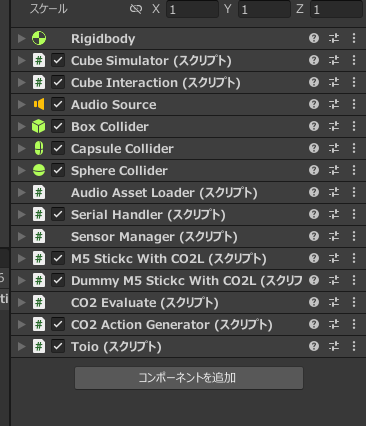
\includegraphics[keepaspectratio, clip, width=0.8\columnwidth]{resources/2024-12-14.png}}
  \caption{}
  \label{fig:}
\end{figure}

早速いいところがあって,コンポーネントで処理を区切ったことで,一部の挙動を変えるのが簡単になった.

土日まるまる使うかと思ってた作業が1日で終わったので,明日は「他者」の評価とそれに伴う快・不快の動作の実装に取り掛かる.

\section*{2024.12.15(日)}
モーションアイデアを考えた.

\fboxsep=0pt            %画像と枠線をくっつける.
\fboxrule=1pt            %枠線の太さを1ptにする.
\begin{figure}[h]
  \centering
  \fbox{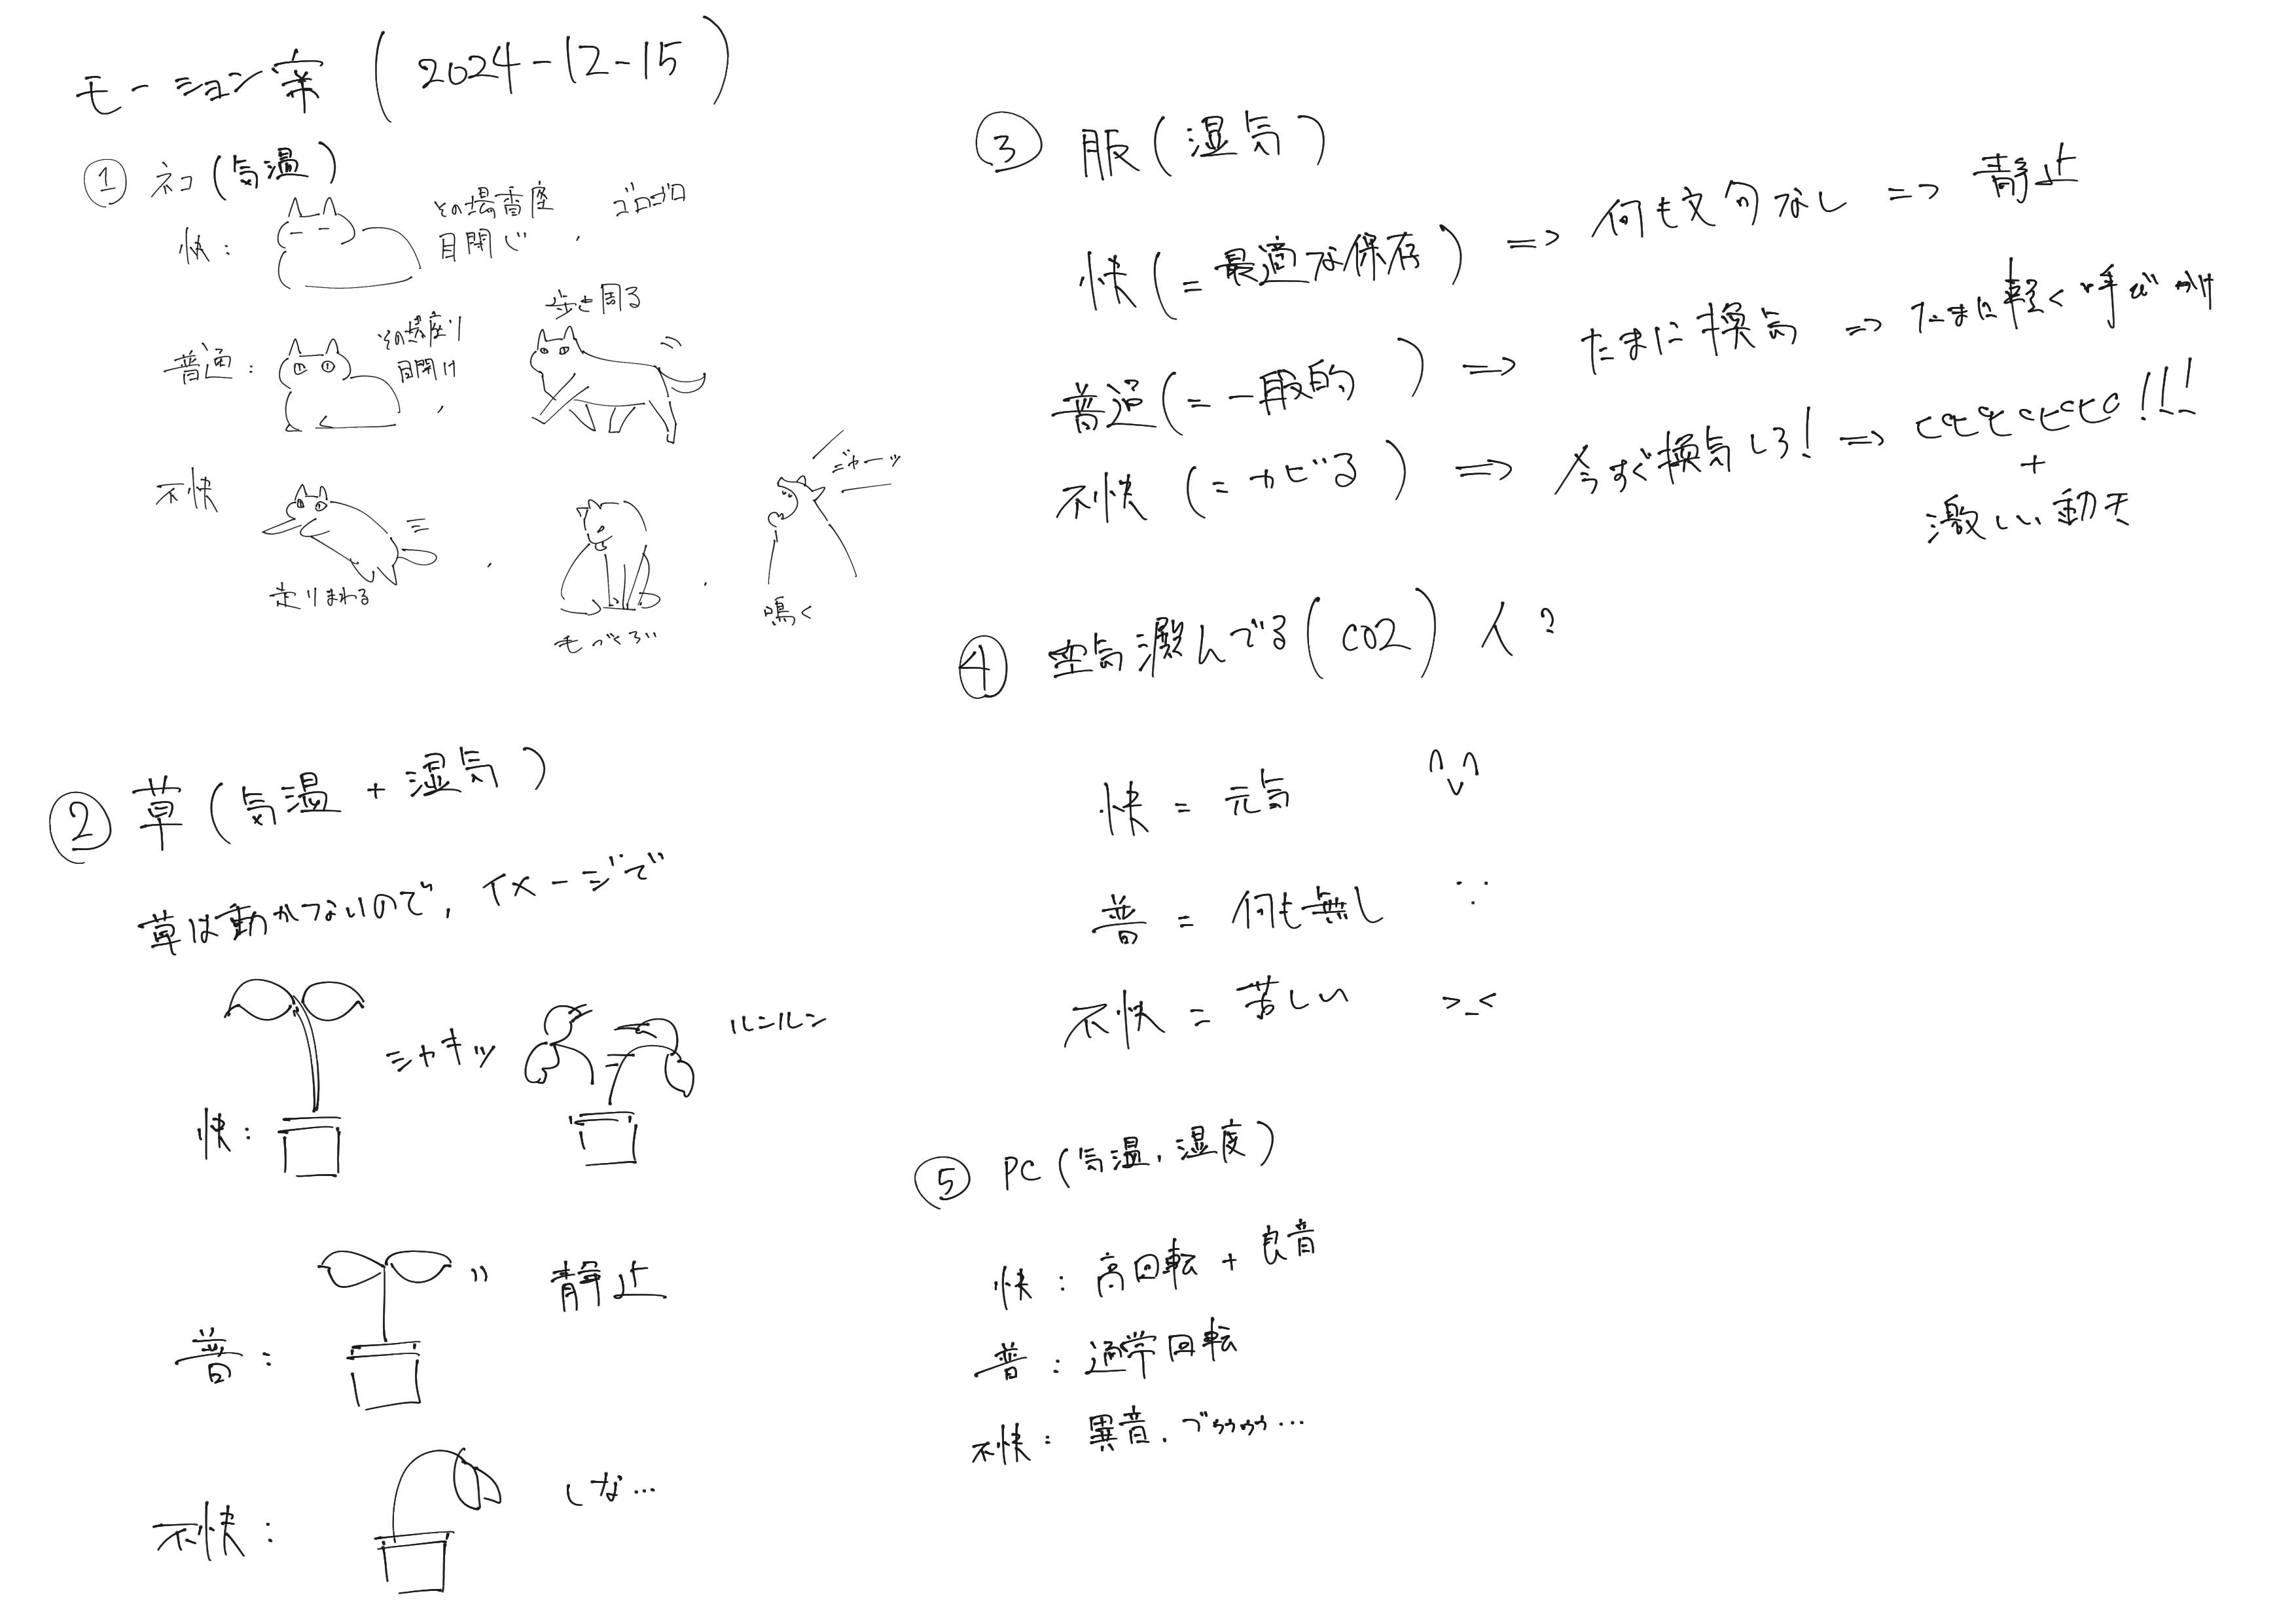
\includegraphics[keepaspectratio, clip, width=0.8\columnwidth]{resources/motion_idea.png}}
  \caption{}
  \label{fig:}
\end{figure}

なんとなくやってたけど,「最適」「危険」じゃなくて,「快.不快」だったね.モンハンの「通常・怒り・疲労」みたいなステート分けになってちょっと面白い.

モンハンの流れでいくなら,モーションも1個1個各ジェネレータでつくるんじゃなくて,ある程度のモーションのまとまりをライブラリにして簡単に生成できるようにしたいな.

\fboxsep=0pt            %画像と枠線をくっつける.
\fboxrule=1pt            %枠線の太さを1ptにする.
\begin{figure}[h]
  \centering
  \fbox{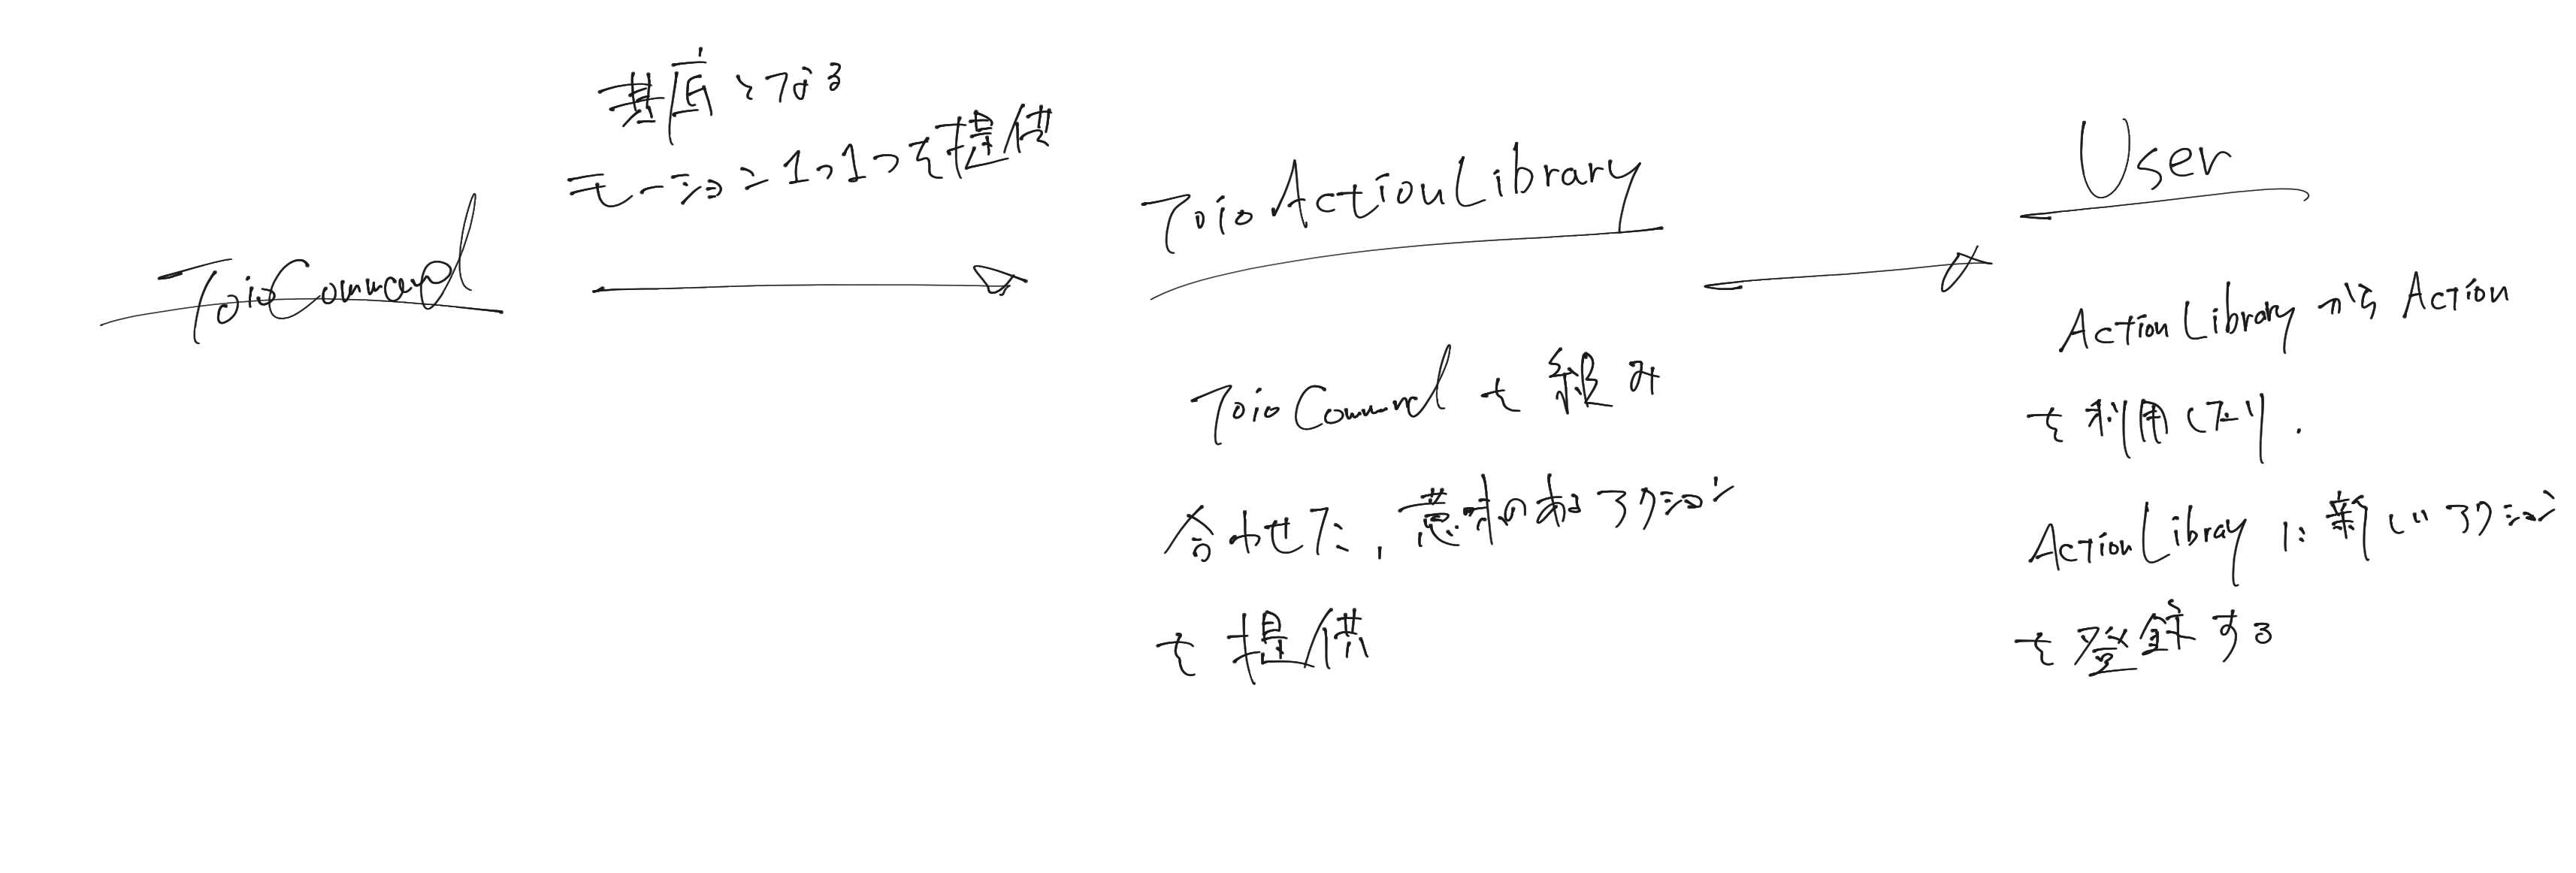
\includegraphics[keepaspectratio, clip, width=0.8\columnwidth]{resources/action_design_flow.png}}
  \caption{}
  \label{fig:}
\end{figure}

\section*{2024.12.15(日)}
AIを使ってとりあえずの評価とモーションを作った.猫気温,草湿度,人間CO2,PC環境,服湿度の5つ.

評価系はともかく,アクションの実行系に課題が見つかった.

現在はアクションをまとめて一つのフォーマットで出力して,Toioのキューで処理しているんだけど,こうすると「ライトつけながら動く」みたいな並列処理ができない.

これを解決するために,今後はモーター使う動き,LED,スピーカーと,使う場所に分けてアクションキューをつくる.

ただ,ある程度形にできたのは確かなので,これはこれで一旦Pushして見せられるものに入れておこう.

\section*{エラー集}
\subsection*{Adafruit BMP280 not found}
ENV用のサンプルスケッチを使うには別途「Adafruit BMP280 Library」のインストールが必要。Arduino IDEのライブラリマネージャーからDLしたら解決

\subsection*{プログラムなんも間違ってないのに\\Arduino IDEのコンパイルに失敗する}
M5StickCのボードはM5StackとESP32っていう2つのグループから出てるんだけども、なにかアプデがあったようで、周辺ライブラリ全体がM5Stack版のM5StickCボードに合わせて構成されるようになった。

なのでESP32を使うとデータ合わなくてライブラリと競合する。間違えるのが心配ならESP32版は消して、M5Stack版だけを残すとよい。

\subsection*{ENV使ってみたいのにサンプルプログラムが動いてくれない!}
どうやらENV2から中身の基盤がSHT3xっていう規格のものに変わったようで、サンプルのDHT12クラスではアクセスができない。

\href{https://qiita.com/visyeii/items/e28f8500f43166710664}{この記事}のプログラムだと行けなくもないけど、また最近変数とかメソッド名が変わったようで、書き換えが必要。まあSHT3xに続けてドット打てばヒントは出てくるので、tempとかhumidとか打てば該当のものは出てくる。

\subsection*{SHT3x入れたのにENV2が機能しない}
そのライブラリ、SHT3"X"じゃありませんか?こっちでも機能する可能性はあるけど、上のリンクで使ってるのは3Xじゃなくて3"x"です。紛らわしいんじゃ。

\subsection*{SHT3"x"をちゃんと入れたのに機能しない}
確証があるわけじゃないけど、bmeの初期化の仕方に問題があるかも。

はじめはsetupでif(bme初期化できてないならエラー出力)って感じだったんだけど、それをwhile(初期化完了するまで)にしたらうまく行った。もしかするとenvはsht3xとbmeがどっちもちゃんと初期化できないと機能しないのかもしれない。

\bibliographystyle{junsrt}
\bibliography{ref}
\end{document}
